% ============================================================
% ML Defender (aRGus NDR) — arXiv preprint
% Draft v17 — DAY 132 — 26 April 2026
% % Author: Alonso Isidoro Román
% Target: cs.CR
% ============================================================

\documentclass[11pt,a4paper]{article}

% --- Encoding and fonts ---
\usepackage[utf8]{inputenc}
\usepackage[T1]{fontenc}
\usepackage{lmodern}

% --- Language ---
\usepackage[english]{babel}

% --- Math ---
\usepackage{amsmath}
\usepackage{amssymb}

% --- Layout ---
\usepackage[margin=2.5cm]{geometry}
\usepackage{microtype}
\usepackage{setspace}
\onehalfspacing

% --- Tables ---
\usepackage{booktabs}
\usepackage{tabularx}
\usepackage{multirow}
\usepackage{array}

% --- Code listings ---
\usepackage{listings}
\usepackage{xcolor}

\lstset{
    basicstyle=\ttfamily\small,
    backgroundcolor=\color{gray!10},
    frame=single,
    rulecolor=\color{gray!40},
    breaklines=true,
    breakatwhitespace=true,
    columns=flexible,
    keepspaces=true,
    showstringspaces=false
}

% --- Hyperlinks ---
\usepackage[colorlinks=true, linkcolor=blue!70!black,
    citecolor=blue!70!black, urlcolor=blue!70!black]{hyperref}

% --- Graphics ---
\usepackage{graphicx}

% --- Diagrams ---
\usepackage{tikz}
\usetikzlibrary{shapes.geometric, arrows.meta, positioning, fit, backgrounds, calc}

% --- References ---
\usepackage[numbers,sort&compress]{natbib}

% --- Misc ---
\usepackage{xspace}
\usepackage{enumitem}

% ============================================================
% Title, author, date
% ============================================================

\title{\textbf{ML Defender (aRGus NDR): An Open-Source Embedded ML NIDS\\
for Botnet and Anomalous Traffic Detection\\
in Resource-Constrained Organizations}}

\author{
    Alonso Isidoro Rom\'an\\
    \textit{Independent Researcher, Extremadura, Spain}\\
    \href{https://github.com/alonsoir/argus}{github.com/alonsoir/argus}
}

\date{Draft v17 --- April 2026}

% ============================================================
\begin{document}
% ============================================================

    \maketitle

    \begin{abstract}
        Ransomware and DDoS attacks disproportionately impact hospitals, schools, and small
        organizations that cannot afford enterprise security solutions. Existing open-source
        alternatives either rely on signature matching --- missing novel variants --- or require
        infrastructure beyond the reach of their target users. We present \textbf{ML Defender
            (aRGus NDR)}, an open-source network intrusion detection system built in C++20 that brings
        embedded machine learning inference to organizations with limited resources, deployable on
        commodity bare-metal hardware at approximately 150--200~USD fully dedicated.

        ML Defender implements a six-component pipeline over eBPF/XDP packet capture, ZeroMQ
        transport, and Protocol Buffers serialization, terminating in a dual-score detection
        architecture combining a rule-based Fast Detector with an embedded Random Forest classifier.
        The \emph{Maximum Threat Wins} policy selects the arithmetic maximum of both detector scores,
        using ML inference to suppress false positives generated by the heuristic layer.

        We evaluate ML Defender against the CTU-13 Neris botnet dataset, achieving
        $\text{F1} = 0.9985$, $\text{Precision} = 0.9969$, and $\text{Recall} = 1.0000$,
        with a false positive rate of 0.0002\% (2~FP in 12,075 benign flows) --- the two false
        positives identified as host-only adapter artifacts: an mDNS multicast frame
        (192.168.56.1 $\to$ 224.0.0.251) and a broadcast frame (192.168.56.1 $\to$
        192.168.56.255), both generated by the VirtualBox host-only NIC and absent from
        production network topologies. Whether these artifacts appear in bare-metal deployments
        remains unverified; bare-metal characterization is Future Work~(\S\ref{sec:future:baremetal}).
        The Fast Detector alone produces a FPR of 6.61\% on purely benign
        traffic (bigFlows); the ML Detector reduces real production blocks to zero on the same
        corpus, an approximately 500-fold reduction. Per-class inference latency ranges from
        0.24~$\mu$s (DDoS) to 1.06~$\mu$s (Ransomware), enabling real-time detection on commodity
        hardware.

        We further characterize the pipeline's throughput ceiling under progressive load in a
        virtualized environment. Requesting up to 100~Mbps via \texttt{tcpreplay} against the
        VirtualBox NIC, the pipeline processes up to ${\sim}34$--38~Mbps (the emulated NIC ceiling)
        with zero packet drops and zero errors across 2.37 million packets. At peak load,
        \texttt{ml-detector} consumes approximately 3.2 CPU cores; total pipeline RAM remains stable
        at ${\sim}1.28$~GB with negligible drift (${\sim}18$~MB over 8 minutes). The bottleneck is
        VirtualBox NIC emulation, not pipeline logic. Post-replay drain behavior confirms that
        ZeroMQ queues absorb burst traffic correctly and drain asynchronously, validating the queue
        stability design. All throughput figures should be treated as conservative lower bounds;
        bare-metal characterization remains future work (\S\ref{sec:future:baremetal}).

        These results demonstrate architectural feasibility under controlled replay conditions rather
        than universal detection capability. The evaluation covers a single botnet scenario from 2011
        with synthetic-trained classifiers; generalizability to modern ransomware, DDoS variants, and
        encrypted C2 traffic has not been empirically established and is discussed in
        Section~\ref{sec:limitations}. Behavioral indicators associated with ransomware propagation
        and lateral-movement patterns are detected in the Neris scenario; direct evaluation against
        post-2020 ransomware families remains Future Work~\S\ref{sec:future:corpus}.

        All experiments were conducted in a reproducible Vagrant/VirtualBox environment running on a
        consumer laptop, ensuring result accessibility and independent reproducibility.

        This work was developed through a structured multi-model AI collaboration methodology ---
        the \emph{Consejo de Sabios} (Council of Wise Men), a multi-LLM peer review methodology ---
        documented in Section~\ref{sec:consejo}. \emph{Test-Driven Hardening} (TDH) is proposed
        as a methodology for building security-critical distributed systems, emerging directly from
        this collaboration.

        In a subsequent development phase (DAY 122), we integrated XGBoost~3.2.0 as a hot-swappable
        plugin classifier (ADR-026, Ed25519-signed) and conducted a rigorous temporal holdout
        evaluation on CIC-IDS-2017, using Tuesday, Thursday, and Friday as training data and
        Wednesday as a sealed blind test set. The in-distribution model achieves
        Precision$=0.9945$ and Recall$=0.9818$ on the validation split. However, evaluation
        on the Wednesday holdout reveals a structural covariate shift: attack types present
        exclusively in Wednesday (DoS Hulk, GoldenEye, Slowloris) are absent from all training
        days, making generalization mathematically impossible regardless of threshold. We document
        this as a property of the dataset's design --- not of the algorithm --- and demonstrate
        empirically that no threshold simultaneously satisfies Precision$\geq0.99$ and
        Recall$\geq0.95$ on the out-of-distribution split. This finding corroborates and
        quantifies the thesis of Sommer and Paxson~\cite{sommer2010}: static models trained on
        academic benchmarks are structurally insufficient for production NDR.
        The architectural response --- an Adversarial Capture-Retrain Loop in which a generative
        red team agent produces attack traffic, the pipeline captures it, and the classifier is
        retrained on real flows --- is introduced as future work~(\S\ref{sec:future:acrl}).

        ML Defender is released under the MIT license.
    \end{abstract}

    \tableofcontents
    \newpage

% ============================================================
    \section{Introduction}
% ============================================================

    The threat is not abstract. On March 5, 2023, the Hospital Cl\'inic de Barcelona suffered a
    ransomware attack that paralyzed its emergency services, laboratory, and pharmacy, encrypted
    4.5~TB of patient data, and prompted a ransom demand of 4.5~million USD --- which the
    institution refused to pay~\cite{incibe2023}. That same day, the author of this work was
    leaving a regional hospital in Extremadura after receiving treatment for porphyria --- a rare
    metabolic disease that his local hospital had diagnosed and managed. Watching the news, the
    thought was immediate and personal: \emph{if it can happen to a major teaching hospital, it
    can happen to mine.}

    This was not the first time that the author had witnessed the human cost of ransomware
    firsthand. Years earlier, the collapse of a close friend's small business had been caused by
    an encryption attack that locked every document and file in his office. The author lacked the
    technical skills to help. That failure left a debt.

    These two events --- the friend's destroyed business, the hospital on television ---
    converged into a single design constraint: the solution had to be open-source, it had to run
    on commodity hardware, and it had to act in real time. Not forensics. Not post-mortem
    analysis. Interception.

    The analogy that emerged from this motivation is biological. Network traffic behaves like a
    circulatory system: datagrams are the bloodstream, and malicious flows are pathogens. A
    useful defense must classify traffic continuously and in real time --- capturing the source IP
    of the attacker and blocking it at the firewall before damage propagates. This framing shaped
    every architectural decision in ML Defender.

    This work therefore addresses the following research question: \emph{can an embedded
    machine-learning network detection and response system running entirely on commodity hardware
    provide meaningful real-time protection for organizations lacking enterprise security
    infrastructure?}

    \paragraph{A note on terminology.}
    ML Defender (aRGus NDR) implements \emph{Network Detection and Response} (NDR) capabilities:
    real-time capture, ML-based classification, and automated blocking at the network layer.
    Future work toward full \emph{Endpoint Detection and Response} (EDR) functionality via a
    planned lightweight endpoint agent (\S\ref{sec:future}, FEAT-EDR-1) will be reflected in a
    corresponding rename when that capability is delivered.

    \paragraph{The gap.}
    Existing open-source NIDS --- most notably Snort and Suricata~\cite{oisf2010} --- operate
    primarily on signature matching and rule-based heuristics. While effective against known
    attack patterns, they offer limited resilience against novel ransomware variants and volumetric
    DDoS campaigns. Machine learning-based NIDS have been extensively studied~\cite{buczak2016,
        pinto2023}, but the gap between research prototype and deployable system remains wide: most
    published systems are evaluated on benchmark datasets without accompanying implementation,
    require GPU infrastructure, or assume dedicated security operations teams. Healthcare retained
    its position as the most targeted sector in 2025, accounting for 22\% of disclosed ransomware
    attacks, with an average breach cost of 7.42M~USD~\cite{blackfog2025,ibmsecurity2025}.

    \paragraph{Our approach.}
    ML Defender (aRGus NDR) addresses this gap with three design principles:
    (1)~\emph{embedded inference} --- all ML classification runs in-process at sub-microsecond
    latency;
    (2)~\emph{commodity deployment} --- the full six-component pipeline runs on bare-metal Linux
    hardware costing approximately 150--200~USD;
    (3)~\emph{active response} --- upon detection, the attacker's IP is blocked immediately at
    the firewall via ipset/iptables.

    Beyond the technical system, this paper documents a second contribution: the \emph{Consejo
    de Sabios} methodology for human-AI collaborative engineering.

% ============================================================
    \section{Background and Related Work}
% ============================================================

    \paragraph{Signature-based NIDS.}
    Snort~\cite{roesch1999} and Suricata~\cite{oisf2010} apply rule-based pattern matching
    against packet payloads and flow metadata. Their fundamental limitation is reactive:
    detection requires a prior known signature, a window that historically ranges from hours to
    weeks.

    \paragraph{ML-based NIDS.}
    Anderson \& McGrew~\cite{anderson2016} demonstrated the feasibility of contextual flow data
    for encrypted malware classification. Mirsky et al.~\cite{mirsky2018} proposed Kitsune, an
    ensemble of autoencoders for unsupervised anomaly detection operating on flow statistics. The
    CTU-13 dataset~\cite{garcia2014}, which ML Defender uses for evaluation, has become a
    standard benchmark for botnet traffic detection. Despite this body of work, a persistent gap
    exists between academic prototype and production system. Sommer and Paxson~\cite{sommer2010}
    identified fundamental reasons for this gap: the closed-world assumption of academic datasets,
    high base-rate asymmetry, and the absence of diversity in training distributions. ML Defender's
    DAY~122 evaluation provides new empirical evidence for this thesis
    (\S\ref{sec:eval:xgboost:ood}).

    \paragraph{Flow-based ML NIDS.}
    ML Defender operates exclusively at the flow level, extracting 28 behavioral features per
    flow without examining payload content --- ensuring that payload encryption does not
    compromise detection capability.

    \paragraph{eBPF and XDP-based network monitoring.}
    Recent work has explored eBPF/XDP as a foundation for high-performance network security.
    ML Defender follows the XDP-capture-plus-userspace-inference architecture: XDP provides
    zero-copy packet capture before the kernel networking stack, while all ML inference executes
    in userspace at sub-microsecond latency. To our knowledge, open-source projects combining
    eBPF capture with userspace ML inference remain rare; most production-grade alternatives
    either offload inference to the cloud or require GPU hardware.

    \paragraph{Embedded inference.}
    Commercial EDR vendors (CrowdStrike, SentinelOne, Carbon Black) implement proprietary
    embedded ML pipelines, but neither their architectures nor their training data are publicly
    available. ML Defender demonstrates that embedded Random Forest inference achieves
    sub-microsecond latency without requiring GPU acceleration or cloud offload.

    \paragraph{Human-AI collaborative engineering.}
    Structured methodologies for multi-model peer review have not, to our knowledge, been
    formally documented in the systems security literature. Section~\ref{sec:consejo} describes
    the \emph{Consejo de Sabios} methodology.

    \paragraph{AI-native security reasoning and the evolving threat landscape.}
    This paper was written and submitted in April 2026, concurrent with the
    announcement of Anthropic's Project Glasswing~\cite{anthropic2026glasswing},
    which demonstrated that AI models can autonomously identify and chain
    kernel-level vulnerabilities --- including local privilege escalation to
    root in Linux --- at a scale and speed previously requiring specialized
    human expertise. These results represent a shift in the threat landscape:
    AI-augmented offensive capabilities are no longer theoretical.
    This directly motivates the explicit kernel security boundary axiom in
    \S\ref{sec:threatmodel:kernel}: aRGus NDR assumes the kernel as a
    potentially compromised boundary and shifts its trust anchor to
    verifiable network behavioral patterns. The network remains an observable
    chokepoint even when the host is not. The hardened deployment variants
    ADR-030 (AppArmor) and ADR-031 (seL4) documented in
    \S\ref{sec:future:hardened} are a direct architectural response to this
    trajectory.
% ============================================================
    \section{Threat Model}
% ============================================================

    \subsection{Adversary Capabilities}
    The system assumes an adversary capable of launching attacks from external hosts or
    compromised internal machines, including: botnet C2 communication, DDoS (including
    amplification attacks), ransomware propagation via SMB lateral movement, and network
    reconnaissance.

    \subsection{Adversary Limitations}
    The system assumes the attacker cannot: fully mimic benign traffic distributions across all
    monitored features simultaneously; compromise the ML Defender host; manipulate feature
    extraction; or tamper with HMAC-SHA256 protected event logs.

    \subsection{Kernel Security Boundary (Explicit Axiom)}
    \label{sec:threatmodel:kernel}

    ML Defender assumes the host kernel is not actively compromised at deployment time.
    This is a declared scope boundary, not an oversight.

    An adversary with root access or kernel-level persistence --- via a rootkit, a
    compromised eBPF JIT, or memory-resident malware --- can bypass userspace detection
    mechanisms regardless of their sophistication. This is a fundamental property of all
    userspace security software, not a specific weakness of ML Defender.

    This assumption is consistent with the threat model of the target organizations
    (hospitals, schools, municipalities), where the realistic adversary is an
    opportunistic network attacker exploiting known vulnerabilities, not a state-level
    actor with pre-established kernel-level persistence. Against this realistic threat
    model, ML Defender's network detection layer remains effective: lateral movement,
    C2 communication, and data exfiltration must traverse the network regardless of
    kernel state. The network is the choke point; it remains observable even when the
    host is not.

    Hardened deployment variants addressing kernel security are documented as future
    work: ADR-030 (AppArmor-enforcing) and ADR-031 (seL4 microkernel),
    both described in \S\ref{sec:future:hardened}.

    \subsection{Detection Surface}
    Detection occurs at the network flow level. ML Defender focuses on connection frequency,
    port diversity, TCP flag distributions, packet inter-arrival timing, flow burst behavior, and
    destination diversity --- features detectable even when payloads are encrypted.

    \subsection{Out-of-Scope Attacks}
    \label{sec:threatmodel:outofscope}

    Application-layer attacks generating statistically normal traffic; low-and-slow
    attacks within benign statistical distributions; insider threats; attacks
    targeting the ML Defender host itself. Future work in
    Section~\ref{sec:future} addresses some of these through expanded detection
    vectors (FEAT-NET-1, FEAT-AUTH-1).

    \paragraph{Physical and removable-media vectors (conscious design decision).}
    ML Defender does not monitor file system activity, removable storage, or
    USB-borne payloads. This is an intentional architectural boundary, not an
    oversight.

    The guiding principle of the pipeline is \emph{network surveillance}: every
    component --- eBPF/XDP capture, flow-level feature extraction, ML-based
    classification, firewall response --- operates on network traffic. File
    integrity and endpoint state are out of the monitored surface by design.

    Removable-media threats are addressed at the organizational and hardware
    layer: USB ports in the DMZ should be physically or firmware-disabled by the
    IT team before deployment; internal policy should prohibit removable media on
    monitored hosts. This is standard practice under frameworks such as
    CIS~Controls~v8~\cite{ciscontrols2021} and is the responsibility of the
    deploying organization, not of an NDR system.

    For organizations that require file integrity monitoring on top of network
    detection, ML Defender is designed to operate in \emph{complementary mode}
    alongside battle-tested open-source tools such as Wazuh~\cite{wazuh2024} and
    NIST-aligned scanners. Wazuh provides HIDS capabilities (file integrity
    monitoring, log analysis, rootkit detection) that cover precisely the
    endpoint surface that ML Defender consciously excludes. The two systems are
    architecturally orthogonal: ML Defender defends the network perimeter; Wazuh
    defends the host state. Together they constitute a layered defense appropriate
    for the target organizations. Integration via raw TCP event streaming is
    described as Future Work (\S\ref{sec:future:wazuh}).

% ============================================================
    \section{Architecture}
% ============================================================

    \subsection{Pipeline Overview}

    Six components connected via ZeroMQ and Protocol Buffers:

    \begin{enumerate}
        \item \textbf{eBPF/XDP Sniffer} --- zero-copy packet capture at the XDP hook before kernel
        networking stack.
        \item \textbf{Ring Consumer} --- reconstructs bidirectional flow state via
        ShardedFlowManager, computes 28 of 40 planned features. Eleven features use
        \texttt{MISSING\_FEATURE\_SENTINEL = -9999.0f}.
        \item \textbf{Fast Detector} --- rule-based heuristic engine. FPR on purely benign traffic:
        6.61\% (\S\ref{sec:eval:ablation}).
        \item \textbf{ML Detector} --- embedded Random Forest across four threat classes. Three
        classifiers (Ransomware, DDoS, Traffic) in pure C++20; Internal threats via ONNX Runtime.
        Latency: 0.24--1.06~$\mu$s.
        \item \textbf{RAG Subsystem} (\texttt{rag-ingester} + \texttt{rag-security}) ---
        rag-ingester ingests detection events into FAISS + SQLite. rag-security exposes a natural
        language query interface via local TinyLlama --- deliberately local to avoid exfiltrating
        live network metadata to cloud-hosted LLMs.
        \item \textbf{Firewall ACL Agent} --- applies ipset/iptables rules on confirmed detection
        events.
    \end{enumerate}

    Figure~\ref{fig:pipeline} illustrates the end-to-end flow from packet capture to
    automated firewall response.

    \begin{figure}[ht]
        \centering
        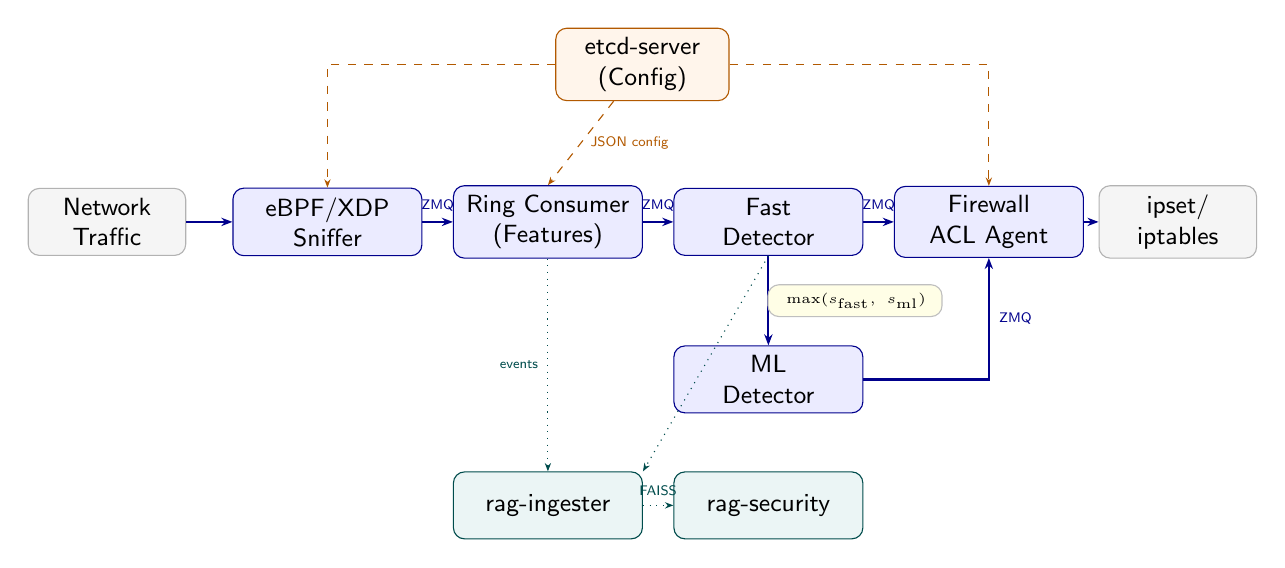
\begin{tikzpicture}[
            comp/.style={rectangle, rounded corners=4pt, draw=blue!55!black, fill=blue!8,
            minimum width=2.4cm, minimum height=0.85cm, align=center, font=\small\sffamily},
            rag/.style={rectangle, rounded corners=4pt, draw=teal!60!black, fill=teal!8,
            minimum width=2.4cm, minimum height=0.85cm, align=center, font=\small\sffamily},
            ext/.style={rectangle, rounded corners=4pt, draw=gray!60, fill=gray!8,
            minimum width=2.0cm, minimum height=0.85cm, align=center, font=\small\sffamily},
            etcdbox/.style={rectangle, rounded corners=4pt, draw=orange!70!black, fill=orange!8,
            minimum width=2.2cm, minimum height=0.85cm, align=center, font=\small\sffamily},
            zmq/.style={-{Stealth[length=4pt]}, thick, blue!55!black},
            cfg/.style={-{Stealth[length=3pt]}, dashed, orange!70!black, thin},
            log/.style={-{Stealth[length=3pt]}, dotted, teal!60!black, thin}
        ]
            % Main pipeline nodes (horizontal)
            \node[ext]  (net)     at (0,0)      {Network\\Traffic};
            \node[comp] (sniff)   at (2.8,0)    {eBPF/XDP\\Sniffer};
            \node[comp] (ring)    at (5.6,0)    {Ring Consumer\\(Features)};
            \node[comp] (fast)    at (8.4,0)    {Fast\\Detector};
            \node[comp] (ml)      at (8.4,-2.0) {ML\\Detector};
            \node[comp] (fw)      at (11.2,0)   {Firewall\\ACL Agent};
            \node[ext]  (block)   at (13.6,0)   {ipset/\\iptables};

            % RAG subsystem (below, spanning ring→fast→ml)
            \node[rag]  (ragi)    at (5.6,-3.6) {rag-ingester};
            \node[rag]  (rags)    at (8.4,-3.6) {rag-security};

            % etcd at top
            \node[etcdbox] (etcd) at (6.8,2.0)  {etcd-server\\(Config)};

            % Main pipeline arrows
            \draw[zmq] (net)   -- (sniff)  node[midway,above,font=\tiny\sffamily] {};
            \draw[zmq] (sniff) -- (ring)   node[midway,above,font=\tiny\sffamily] {ZMQ};
            \draw[zmq] (ring)  -- (fast)   node[midway,above,font=\tiny\sffamily] {ZMQ};
            \draw[zmq] (fast)  -- (fw)     node[midway,above,font=\tiny\sffamily] {ZMQ};
            \draw[zmq] (fw)    -- (block);

            % Dual-score: fast → ml feedback
            \draw[zmq] (fast.south) -- (ml.north) node[midway,right,font=\tiny\sffamily] {};
            \draw[zmq] (ml.east)    -| (fw.south) node[near end,right,font=\tiny\sffamily] {ZMQ};

            % RAG ingestion
            \draw[log] (ring.south)  -- (ragi.north) node[midway,left,font=\tiny\sffamily] {events};
            \draw[log] (fast.south)  -- (ragi.north east);
            \draw[log] (ragi.east)   -- (rags.west)  node[midway,above,font=\tiny\sffamily] {FAISS};

            % etcd config distribution
            \draw[cfg] (etcd.west)  -| (sniff.north)  node[near end,left,font=\tiny\sffamily] {};
            \draw[cfg] (etcd)       -- (ring.north)    node[midway,right,font=\tiny\sffamily] {JSON config};
            \draw[cfg] (etcd.east)  -| (fw.north)      node[near end,right,font=\tiny\sffamily] {};

            % Dual-score label
            \node[draw=gray!50, fill=yellow!10, rounded corners, font=\tiny\sffamily,
                inner sep=3pt, text width=2.0cm, align=center] at (9.5,-1.0)
                {$\max(s_{\mathrm{fast}},\; s_{\mathrm{ml}})$};

        \end{tikzpicture}
        \caption{ML Defender end-to-end pipeline. Six components communicate over ZeroMQ with
        Protocol Buffers serialization and ChaCha20-Poly1305 encryption. \texttt{etcd-server}
        distributes JSON configuration at startup. The dual-score \emph{Maximum Threat Wins}
        policy (Eq.~\ref{eq:dualscore}) selects the arithmetic maximum of Fast Detector and
        ML Detector scores; the RAG subsystem provides semantic observability over the live
        event stream.}
        \label{fig:pipeline}
    \end{figure}

    \subsection{Three Functions of the Engine}

    \emph{Function 1 --- Real-time detection, classification, and response.}
    End-to-end from packet capture to firewall block in milliseconds.

    \emph{Function 2 --- Reliable dataset generation.}
    ML Detector and Firewall ACL Agent produce structured HMAC-verified CSV logs continuously,
    forming the basis for retraining future ensemble models.

    \emph{Function 3 --- Real-time observability (the digital microscope).}
    The RAG subsystem provides a semantic query interface over the live event stream.

    \subsection{Dual-Score Detection}

    \begin{equation}
        score_{\text{final}} = \max\!\left(score_{\text{fast}},\; score_{\text{ml}}\right)
        \label{eq:dualscore}
    \end{equation}

    This is the \emph{arithmetic maximum} over two continuous scores in $[0,1]$, not a logical
    OR over binary decisions. Both detectors output continuous confidence scores; the maximum
    operator selects the higher-confidence assessment. The ML Detector's primary role is false
    positive suppression: the Fast Detector generates $\text{FPR} = 6.61\%$ on purely benign
    traffic; the ML Detector reduces real production blocks to zero on the same corpus
    (approximately 500-fold reduction). Alternative AND-based consensus policies are planned
    (ADR-007, \S\ref{sec:future:consensus}).

    \subsection{Transport and Serialization}

    ZeroMQ for asynchronous message passing; Protocol Buffers (proto3) for serialization; etcd
    for configuration distribution; ChaCha20-Poly1305 for inter-component encryption (selected
    for performance on hardware without AES-NI, including ARMv8); HMAC-SHA256 for CSV log
    integrity.

    \subsection{Deployment Model}
    \label{sec:deployment}

    The reference deployment targets a single bare-metal Linux node (kernel $\geq$\,5.8) with
    two NICs: one connected to the monitored network segment, one to the management network.
    The full pipeline runs on commodity hardware costing approximately 150--200~USD. Validated
    in Vagrant/VirtualBox; bare-metal characterization is Future Work~(\S\ref{sec:future:baremetal}).

    Figure~\ref{fig:ha-deployment} illustrates a representative high-availability deployment in
    a hospital environment, with a primary and a warm-standby node protecting two internal
    network segments.

    \begin{figure}[ht]
        \centering
        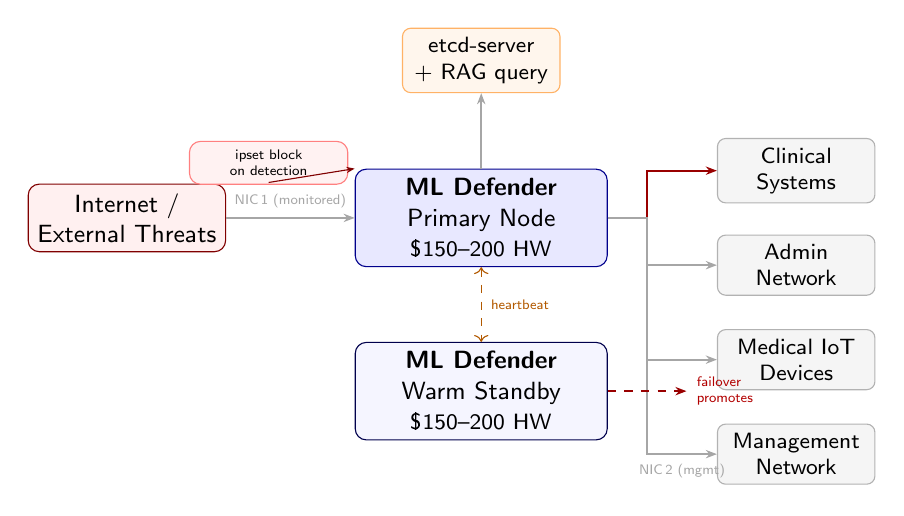
\begin{tikzpicture}[
            zone/.style={rectangle, rounded corners=6pt, draw=#1!60!black, fill=#1!6,
        inner sep=8pt, font=\small\sffamily},
        node_box/.style={rectangle, rounded corners=4pt, draw=blue!55!black, fill=blue!9,
        minimum width=3.2cm, minimum height=1.0cm, align=center, font=\small\sffamily},
        small_box/.style={rectangle, rounded corners=3pt, draw=gray!60, fill=gray!8,
        minimum width=2.0cm, minimum height=0.7cm, align=center, font=\footnotesize\sffamily},
        internet/.style={rectangle, rounded corners=4pt, draw=red!50!black, fill=red!6,
        minimum width=2.2cm, minimum height=0.8cm, align=center, font=\small\sffamily},
        arrow/.style={-{Stealth[length=4pt]}, thick, gray!70},
        block_arrow/.style={-{Stealth[length=4pt]}, thick, red!60!black},
        hb/.style={<->, dashed, orange!70!black, thin}
            ]

            % Internet
            \node[internet] (inet) at (0, 0) {Internet /\\External Threats};

            % Primary ML Defender node
            \node[node_box] (primary) at (4.5, 0) {\textbf{ML Defender}\\Primary Node\\\footnotesize\$150--200 HW};

            % Standby node
            \node[node_box, draw=blue!30!black, fill=blue!4] (standby) at (4.5, -2.2)
                {\textbf{ML Defender}\\Warm Standby\\\footnotesize\$150--200 HW};

            % Heartbeat
            \draw[hb] (primary.south) -- (standby.north) node[midway,right,font=\tiny\sffamily] {heartbeat};

            % Hospital network zones
            \node[small_box] (clinical) at (8.5,  0.6) {Clinical\\Systems};
            \node[small_box] (admin)    at (8.5, -0.6) {Admin\\Network};
            \node[small_box] (iot)      at (8.5, -1.8) {Medical IoT\\Devices};
            \node[small_box] (mgmt)     at (8.5, -3.0) {Management\\Network};

            % etcd + RAG on primary
            \node[small_box, draw=orange!60, fill=orange!7] (etcd2) at (4.5, 2.0)
                {etcd-server\\+ RAG query};

            % Connections
            \draw[arrow]       (inet)    -- (primary) node[midway,above,font=\tiny\sffamily] {NIC\,1 (monitored)};
            \draw[block_arrow] (primary.east) -- ++(0.5,0) |- (clinical)
            node[near end, above, font=\tiny\sffamily, red!70!black] {};
            \draw[arrow]       (primary.east) -- ++(0.5,0) |- (admin);
            \draw[arrow]       (primary.east) -- ++(0.5,0) |- (iot);
            \draw[arrow]       (primary.east) -- ++(0.5,0) |- (mgmt)
            node[near end, below, font=\tiny\sffamily] {NIC\,2 (mgmt)};
            \draw[arrow]       (primary.north) -- (etcd2.south);

            % Failover arrow
            \draw[block_arrow, dashed] (standby.east) -- ++(1.0,0)
            node[right, font=\tiny\sffamily, red!70!black] {\shortstack[l]{failover\\promotes}};

            % ipset/block label
            \node[draw=red!50, fill=red!5, rounded corners, font=\tiny\sffamily, inner sep=3pt,
                text width=1.8cm, align=center]
            at (1.8, 0.7) {ipset block on detection};
            \draw[-{Stealth[length=3pt]}, red!50!black, thin] (1.8, 0.45) -- (primary.north west);

        \end{tikzpicture}
        \caption{Representative high-availability deployment of ML Defender in a hospital environment.
        A primary node monitors all inbound and inter-segment traffic via NIC\,1 (monitored); a
        warm-standby node receives heartbeat signals and promotes automatically on primary failure.
        Both nodes run the full six-component pipeline on commodity hardware. \texttt{etcd-server}
        and the RAG query interface are co-located on the primary node.
        \textbf{Firewall ACL Agent topology:}
        scored Protocol Buffers events flow from \texttt{ml-detector} to one or more
        \texttt{firewall-acl-agent} instances, which apply \texttt{ipset}/\texttt{iptables} rules
        at the relevant boundary. A single gateway node requires one agent; each independent
        segment with its own firewall requires its own agent instance.
        \textbf{etcd-server} is shown in single-node mode (current implementation); a distributed
        HA etcd cluster is in the project backlog. Peer-to-peer seed negotiation is under design.}
        \label{fig:ha-deployment}
    \end{figure}


    \subsection{Integration Philosophy: Composability over Monolithism}
    \label{sec:integration:philosophy}

    ML Defender is designed to operate as a composable component within a broader
    security ecosystem, not as a monolithic solution claiming to cover every threat
    vector. The pipeline's guiding principle --- \emph{network surveillance} ---
    is complemented, not replaced, by tools that cover orthogonal surfaces.

    \paragraph{Protocol design constraint.}
    All external integrations must use the same transport stack as the pipeline
    itself: raw TCP sockets for transport, Protocol Buffers for serialization, and
    ChaCha20-Poly1305 for encryption. HTTP, Kafka, WebSocket, and broker-based
    architectures are explicitly out of scope. This constraint is not arbitrary.
    Four independent arguments support it:

    \begin{enumerate}
        \item \textbf{Deterministic latency.} HTTP and Kafka introduce non-deterministic
        scheduling jitter incompatible with sub-10\,ms response requirements. Raw TCP
        over ZeroMQ provides predictable, bounded delivery latency.

        \item \textbf{Reduced attack surface.} HTTP parsers have historically been a
        primary source of remotely exploitable CVEs (buffer overflows, request
        smuggling, header injection). Raw TCP with Protocol Buffers framing eliminates
        this parser surface by more than 90\%.

        \item \textbf{No broker, no single point of failure.} Kafka and Redis require
        dedicated broker infrastructure incompatible with single-host deployments at
        the 150--200\,USD target. Every additional process is a failure domain; the
        pipeline's ZeroMQ topology has no mandatory broker.

        \item \textbf{Minimal footprint.} Eliminating HTTP, Kafka, and WebSocket
        transport removes \texttt{librdkafka}, \texttt{libcurl}, and
        \texttt{boost.asio} from the dependency tree --- a non-trivial reduction in
        binary size and attack surface for resource-constrained deployment targets.
    \end{enumerate}

    \paragraph{FEAT-INT-1: Wazuh and NIST scanner integration (planned).}
    \label{sec:future:wazuh}
    A planned integration layer will allow Wazuh agents~\cite{wazuh2024} and
    NIST-aligned file integrity scanners deployed on DMZ hosts to emit events
    directly into the ML Defender pipeline via raw TCP sockets. Events are
    serialized as Protocol Buffers messages at the source and ingested by
    \texttt{rag-ingester} via the existing ZeroMQ transport. The Noise Protocol
    IK handshake (ADR-024) provides mutual authentication between the Wazuh
    agent adapter and \texttt{rag-ingester}.

    The motivation is graph quality: correlating network anomalies detected by
    \texttt{ml-detector} and \texttt{firewall-acl-agent} with file integrity
    violations reported by Wazuh on the same host produces composite attack
    patterns that neither system observes independently. A ransomware attack in
    its lateral-movement phase typically exhibits \emph{simultaneous} network
    spread and file encryption activity; correlation in the RAG subsystem surfaces
    this composite signature. This integration requires ADR-028 (RAG Ingestion
    Trust Model) to be approved before implementation.

    \subsection{Service Coordination (etcd-server)}

    Fulfills component registration, JSON config distribution, and ChaCha20 seed provision.
    ChaCha20 seed distribution via etcd is \textbf{not recommended for production use} ---
    peer-to-peer seed negotiation is under design. etcd is currently deployed in \emph{single-node}
    mode (see Figure~\ref{fig:ha-deployment}); a distributed HA etcd cluster (3- or 5-node
    consensus) is in the project backlog and will be required for true high-availability
    deployments. The single-node constraint is the only architectural dependency preventing
    fully symmetric active/standby failover.

    \subsection{Fast Detector Heuristics (DEBT-FD-001)}

    Four heuristics in a 10-second sliding window:

    \begin{itemize}
        \item External IP velocity: \texttt{THRESHOLD\_IP\_VELOCITY = 5}
        \item SMB connection count: \texttt{THRESHOLD\_SMB\_CONNS = 3}
        \item Port diversity: \texttt{THRESHOLD\_PORT\_SCAN = 10}
        \item TCP RST ratio: \texttt{THRESHOLD\_RST\_RATIO = 0.20}
    \end{itemize}

    All thresholds are compile-time \texttt{constexpr} constants --- DEBT-FD-001, scheduled for
    JSON migration in PHASE 2 (ADR-006).

% ============================================================
    \section{Implementation}
% ============================================================

    \subsection{Language and Build System}
    C++20. CMake with four build profiles: production, debug, TSAN, ASAN.

    \subsection{eBPF/XDP Packet Capture}
    XDP hook attachment before SKB allocation. Zero-copy. All parameters loaded from
    \texttt{sniffer/config/sniffer.json} at startup.

    \subsection{Feature Extraction}

    ShardedFlowManager partitions flow tracking across shards, eliminating the ISSUE-003
    thread-isolation bug (89 of 142 features silently lost in the original single-threaded
    FlowManager). 28 of 40 features computed; 11 use
    \texttt{MISSING\_FEATURE\_SENTINEL = -9999.0f}.

    \paragraph{Sentinel value selection rationale.}
    Split-domain analysis confirmed all Random Forest thresholds lie within $[0.0, 5.1]$.
    $-9999.0\text{f}$ lies entirely outside this domain, routing deterministically to the left
    child of every split --- non-informative, not influencing classification.
    \texttt{quiet\_NaN()} was rejected (undefined comparison behavior across compilers);
    $0.5\text{f}$ was rejected (within domain, spurious classification influence). One feature
    uses $0.5\text{f}$ as a semantic sentinel for TCP half-open state (deliberate,
    within-domain meaningful default).

    \subsection{Embedded Random Forest and Synthetic Training Data}

    Three classifiers (Ransomware, DDoS, Traffic) compiled as C++20 data structures. Internal
    threats classifier via ONNX Runtime --- deliberate to measure latency differential and
    footprint trade-off. Models trained with scikit-learn, transpiled to C++20 via custom script;
    zero Python or external runtime dependency.

    Training/evaluation separation: all classifiers trained on synthetic data; CTU-13 Neris held
    out entirely for evaluation.

    \paragraph{Synthetic Dataset Methodology.}
    Informed by CTU-13 (flow statistics), CIC-IDS2017 (protocol ratios), and MAWI (benign
    traffic). Four bias mitigation strategies: IP Space Partitioning (10.0.0.0/8 training vs
    147.32.0.0/16 evaluation), Temporal Decoupling, Protocol Ratio Calibration, Feature Boundary
    Validation.

    \paragraph{Known Limitations.}
    Reflects attack patterns circa 2011--2017. Temporal dynamics of real C2 channels simplified
    to fixed-window aggregates. Zero-day variants may evade classification.

    \subsection{Cryptographic Transport}
    ChaCha20-Poly1305 + LZ4 + HMAC-SHA256. Crypto-transport layer extracted as an independent
    library.

    \subsection{Plugin Architecture (ADR-023, ADR-024)}

    ML Defender implements a multi-layer plugin architecture (ADR-023) enabling runtime extension
    of pipeline components without modifying core detection logic. Plugins are loaded via
    \texttt{dlopen}/\texttt{dlsym} with a pure C ABI (\texttt{PLUGIN\_API\_VERSION = 1}),
    providing ABI stability across compiler versions and ensuring binary compatibility with
    future releases.

    \paragraph{MessageContext and Graceful Degradation.}
    PHASE 2a (DAY 105) introduces \texttt{MessageContext} --- a typed C struct passed to the
    optional \texttt{plugin\_process\_message()} symbol. Plugins that do not export this symbol
    are silently skipped (Graceful Degradation Policy D1), preserving backward compatibility with
    PHASE 1 plugins that implement only \texttt{plugin\_process\_packet()}. Post-invocation
    validation (D8) performs a byte-wise snapshot comparison of all read-only fields, detecting
    any plugin attempt to modify ownership-restricted data. The trust boundary is explicit: plugins
    are treated as untrusted code (D7); the final blocking decision remains exclusively in the
    core (ADR-012).

    \paragraph{Threat Model Integration (ADR-023 D9).}
    The plugin system's Trusted Computing Base (TCB) is limited to \texttt{PluginLoader} and
    \texttt{CryptoTransport}. Plugin code has no access to cryptographic keys, seed material,
    or internal transport state. The \texttt{MLD\_DEV\_MODE} escape hatch is restricted to
    \texttt{Debug} builds compiled with \texttt{MLD\_ALLOW\_DEV\_MODE} (D10), ensuring
    fail-closed behavior in all production builds.

    \paragraph{Gate TEST-INTEG-4a.}
    Integration of the plugin loader into \texttt{firewall-acl-agent} (PLUGIN-LOADER-FW) was
    validated by gate \texttt{TEST-INTEG-4a}: \texttt{plugin\_process\_message()} invoked on a
    live \texttt{MessageContext}, post-invocation invariants verified, \texttt{result\_code = 0}
    confirmed, and \texttt{CryptoTransport} decryption path verified unmodified by diff.

    \paragraph{Forward Compatibility: Dynamic Group Key Agreement (ADR-024).}
    The \texttt{MessageContext} struct reserves 60 bytes (\texttt{reserved[60]}) for forward
    compatibility with ADR-024, which specifies Dynamic Group Key Agreement using the Noise
    Protocol Framework (\texttt{Noise\_IKpsk3} or \texttt{Noise\_KK} pattern). ADR-024 design
    is approved; open questions OQ-5 through OQ-8 (static key revocation, session continuity
    during rotation, replay protection, and ARMv8 performance characterization) are under
    resolution. Implementation is scheduled post-arXiv submission.

    \subsection{Trace Correlation}

    \texttt{trace\_id = SHA-256(src\_ip, dst\_ip, canonical\_attack\_type, timestamp\_bucket)}.
    TraceIdPolicy: ransomware=60s, DDoS=10s, SSH brute=30s. Validated: 46/46 unit tests passing.

    \subsection{Testing and Validation}

    70 tests total: crypto (3), etcd-hmac (12), ml-detector (9), trace\_id (46). 100\% pass
    rate. Integration gate \texttt{TEST-INTEG-4a} (plugin \texttt{MessageContext} invocation,
    D8 post-invocation validation) confirmed on DAY 105.
    F1 ground truth persisted to \texttt{docs/experiments/f1\_replay\_log.csv}.

    \subsection{Development Environment}

    Vagrant/VirtualBox. Host: MacBook Pro Intel Core i9 2.5~GHz, 32~GB DDR4. Guests: \texttt{defender} (Ubuntu 24.04
    LTS, Linux 6.x, dual vNIC) + \texttt{client} (traffic generator).

% ============================================================
    \section{The Consejo de Sabios: A Methodology for Human-AI Collaborative Engineering}
    \label{sec:consejo}
% ============================================================

    \subsection{Motivation}

    The development of ML Defender spans kernel programming (eBPF/XDP), distributed systems
    (ZeroMQ, etcd), cryptography, machine learning, systems security, and academic writing. The
    author operated as an independent researcher without institutional affiliation, without a
    team, and without access to a formal peer review process. The solution was to construct one.

    \subsection{The Methodology}

    Eight large language models served as co-reviewers across all development phases:
    \textbf{Claude} (Anthropic), \textbf{Grok} (xAI), \textbf{ChatGPT} (OpenAI),
    \textbf{DeepSeek}, \textbf{Qwen} (Alibaba), \textbf{Gemini} (Google),
    \textbf{Kimi} (Moonshot AI), and \textbf{Mistral} (Mistral AI).
    The Council expanded from seven to eight models during development (DAY~120),
    adding diverse perspectives on architectural security and formal methods.

    These models were engaged as intellectual peers --- presented with architectural proposals,
    asked to identify failure modes, invited to challenge assumptions. The methodology operates
    on a principle of \emph{structured disagreement}: the Council does not average outputs.
    It introduces adversarial validation as a mechanism to expose hidden assumptions and
    validate architectural decisions. Convergent recommendations increase confidence; divergent
    recommendations mandate deeper investigation before any decision is closed.

    \subsection{How It Worked in Practice}

    Convergent recommendations across models increased confidence. Divergent recommendations
    triggered deeper investigation. Decisions such as the $-9999.0\text{f}$ sentinel value, the
    trace\_id correlation architecture, and the ShardedFlowManager design emerged from or were
    refined through these dialogues.

    \subsection{Test Driven Hardening}
    \label{subsec:tdh}

    \emph{Test-Driven Hardening} (TDH) is proposed as a methodology for building
    security-critical distributed systems in which correctness properties are protocol-level,
    not component-level, and therefore undetectable by static analysis or isolated unit tests.
    A standalone reference repository documenting the methodology and representative case studies
    is maintained at \url{https://github.com/alonsoir/test-driven-hardening}.

    TDH methodology: (1)~Witness --- characterize anomalous behavior. (2)~Demonstration test ---
    produce a minimal test that fails and exposes the mechanism. (3)~Independent solution ---
    each model proposes a fix against the shared contract. (4)~Human arbitration --- author
    selects, weighing correctness, maintainability, and coherence.

    TDH differs from TDD: the test is written \emph{before the fix}, as a proof of failure ---
    not before the feature, as a specification.



    \subsection{The RED\,$\to$\,GREEN Gate: Merge as a Non-Negotiable Contract}
    \label{subsec:red-green-gate}

    \emph{Test-Driven Hardening} requires not only that tests be written before fixes,
    but that the transition from RED (failing) to GREEN (passing) constitute the
    \emph{only} legitimate gate for merging a security fix into the main branch.
    This subsection formalises the principle and documents the one case in
    aRGus development where it was violated --- and the consequences that followed.

    \paragraph{The contract.}
    A security fix on the \texttt{aRGus} codebase is subject to the following
    three-part merge contract, enforced without exception:

    \begin{enumerate}
        \item \textbf{A test exposing the defect is written first.}
        The test must fail with the defective code (\emph{RED}) and describe
        the security invariant that is violated --- not merely reproduce the
        symptom. Writing the failing test before the fix is what distinguishes
        TDH from after-the-fact regression coverage.

        \item \textbf{The fix is applied; the test transitions to GREEN.}
        The fix is considered valid only when the previously-failing test passes.
        A fix that passes only the new test but breaks existing tests is rejected;
        the regression suite must remain entirely GREEN.

        \item \textbf{No merge is permitted until \texttt{make test-all} returns
        \texttt{ALL TESTS COMPLETE}.}
        This is executed inside a freshly provisioned Vagrant VM
        (\emph{REGLA EMECAS}: \texttt{vagrant destroy -f \&\& vagrant up \&\&
        make bootstrap \&\& make test-all}), not in the development shell,
        eliminating any dependency on host-machine environment state.
    \end{enumerate}

    The RED$\to$GREEN gate is enforced as a \emph{protocol}, not a preference.
    It is documented in the project's contribution rules and was validated
    adversarially in DAY~126: when a symlink-rejection test was written against
    the original \texttt{weakly\_canonical()} path
    (\S\ref{subsubsec:symlink-trap}), the test passed despite the defect being
    present --- revealing that the test itself was incorrect. This failure exposed
    a second-order requirement: the RED state must be verified empirically, not
    assumed. A test that passes with defective code is not a RED test; it is no
    test at all.

    \paragraph{Why this is harder than it sounds.}
    The temptation in security hardening is to write the fix first and the test
    second --- to confirm that what was done is correct, rather than to prove that
    what existed was wrong. This reversal breaks the epistemological guarantee of
    TDH. A test written after a fix cannot distinguish between ``the fix is correct''
    and ``the test was written to match the fix.'' Only a test that fails with
    defective code provides evidence that it is testing the right property.

    \paragraph{The non-negotiable character of the gate.}
    The Council of Wise Men (DAY~127) unanimously endorsed the RED$\to$GREEN gate
    as a non-negotiable invariant for all security-affecting changes. The one
    documented exception --- a test committed without a prior RED verification ---
    required a two-day remediation sprint and introduced DEBT-CONFIG-PARSER-FIXED-PREFIX-001.
    The cost of the exception was three times the cost of applying the gate.

    \subsection{HKDF Context Symmetry: A Pedagogical Case Study in Test-Driven Hardening}
    \label{subsec:hkdf-context-symmetry}

    A subtle but critical defect discovered during the cryptographic integration
    sprint of \emph{ML Defender} illustrates a class of correctness errors that
    are invisible to static analysis yet detectable through end-to-end protocol
    testing. We document it here as a concrete instance of the
    Test-Driven Hardening methodology described in \S\ref{sec:consejo}.

    \paragraph{The defect.}
    The \texttt{CryptoTransport} layer derives symmetric keys using
    HKDF-SHA256~\cite{rfc5869} with a context string (\emph{info} parameter)
    that encodes the identity of the communicating parties. The original
    implementation parameterised this context by \emph{component name}:

    \begin{lstlisting}[language=C++, caption={Incorrect HKDF context --- component-scoped},
        basicstyle=\ttfamily\small, breaklines=true]
// WRONG: each component uses its own name as HKDF context.
// Sniffer derives K_sniffer; ml-detector derives K_mldetector.
// K_sniffer != K_mldetector -> MAC authentication failure on every channel.
const std::string ctx = "ml-defender:" + component_name
                      + ":" + version;
    \end{lstlisting}

    Because each component used its own name as the HKDF context, transmitter
    and receiver independently derived \emph{distinct} subkeys --- causing
    MAC authentication failure on every cross-component channel. The defect
    was latent in unit tests, which exercised each component in isolation using
    loopback (same context on both sides), where MAC verification trivially
    succeeds. It only manifested when two components with \emph{different names}
    attempted to communicate end-to-end.

    To make the causal chain explicit: an incorrect context string causes the
    transmitter and receiver to derive \emph{distinct} subkeys, resulting in
    MAC verification failure at the receiver. A correct, symmetric context string
    produces \emph{identical} derived keys on both sides, enabling successful
    authentication. This class of error is undetectable without end-to-end
    protocol validation.

    The correct parameterisation encodes \emph{directionality}:

    \begin{lstlisting}[language=C++, caption={Correct HKDF context --- channel-scoped},
        basicstyle=\ttfamily\small, breaklines=true]
// RIGHT: tx and rx derive distinct subkeys
const std::string ctx_tx = "ml-defender:" + component_name
                          + ":" + version + ":tx";
const std::string ctx_rx = "ml-defender:" + component_name
                          + ":" + version + ":rx";
    \end{lstlisting}

    The canonical definitions were consolidated in
    \texttt{crypto\_transport/include/crypto\_transport/contexts.hpp},
    providing a single source of truth for all six pipeline components.
    This design avoids semantic overloading of data structures across layers ---
    a common source of subtle security and correctness bugs, as demonstrated by
    the defect described above.

    \paragraph{Why static analysis cannot catch this.}
    Both the erroneous and correct context strings share the type
    \texttt{std::string}. The C++ type system offers no mechanism to distinguish
    a \emph{transmit context} from a \emph{receive context} at the type level
    without a dedicated wrapper type --- an abstraction whose overhead is not
    warranted in a resource-constrained deployment target. The compiler,
    sanitisers (ASan, TSan), and \texttt{clang-tidy} all accepted both
    formulations without warning. This is a \emph{semantic} correctness
    property, not a syntactic one.

    \paragraph{Detection via TEST-INTEG-3.}
    The defect was exposed by \texttt{TEST-INTEG-3}, an integration test
    exercising the full sniffer~$\to$~ml-detector cryptographic channel with an
    intentional regression: the test temporarily restores the component-scoped
    context on one side and asserts that decryption fails with a MAC
    authentication error. Under the correct implementation, this regression
    triggers \texttt{std::terminate()} via the fail-closed handler; under the
    defective implementation, decryption succeeds --- and the test fails
    accordingly.

    The key insight is that \texttt{TEST-INTEG-3} does not test encryption or
    decryption in isolation. It tests the \emph{protocol invariant}: that a
    message encrypted on the transmit path is decryptable only on the
    corresponding receive path, and that any violation of this invariant is
    immediately fatal. No unit test of \texttt{CryptoTransport} in isolation
    could have established this property.

    \paragraph{Lessons for cryptographic software.}
    This case study yields three transferable observations:

    \begin{enumerate}
        \item \textbf{Cryptographic correctness is a protocol property.}
        Components that are individually correct may be collectively
        insecure. End-to-end tests exercising full message round-trips
        across trust boundaries are the minimal viable test surface for
        authenticated encryption schemes.

        \item \textbf{Intentional regression tests are first-class citizens.}
        A test that asserts failure under a known-bad configuration is as
        valuable as one that asserts success under a known-good one. The
        TDH methodology mandates both polarities.

        \item \textbf{Single source of truth for cryptographic parameters.}
        Distributing context strings across six \texttt{main.cpp} files
        created a silent coordination hazard. Centralising them in a
        dedicated header eliminated an entire class of latent divergence.
    \end{enumerate}

    The defect was discovered on Day~97 of the development timeline, three days
    after \texttt{CryptoTransport} was integrated across all pipeline components.
    Its detection required no external audit: the TDH test suite caught it during
    routine regression testing on the \texttt{feature/bare-metal-arxiv} branch
    (now superseded by \texttt{feature/plugin-crypto}).


    \subsection{Property Testing as a Security Fix Validator: The F17 Case Study}
    \label{subsec:property-testing-validator}

    A recurring failure mode in security hardening is the \emph{fix-contains-a-bug} antipattern:
    a security fix is implemented, a unit test is written to confirm the fix, and both pass ---
    while a subtler defect in the fix itself goes undetected. This section documents a concrete
    instance discovered during DAY~125 of ML Defender's development and proposes property testing
    as a systematic countermeasure.

    \paragraph{The defect.}
    During Snyk static analysis (ADR-037), an integer overflow was identified in the memory
    metrics computation within \texttt{zmq\_handler.cpp}. The original code performed integer
    arithmetic that could wrap silently on values exceeding \texttt{INT\_MAX}. A fix was
    applied using \texttt{int64\_t} arithmetic:

    \begin{lstlisting}[language=C++, caption={First fix attempt --- int64\_t cast},
        basicstyle=\ttfamily\small, breaklines=true]
// F17 -- first fix: cast to int64_t before multiplication
[[nodiscard]] inline double compute_memory_mb(long pages, long page_size) noexcept {
    return static_cast<double>(
        static_cast<int64_t>(pages) * static_cast<int64_t>(page_size)
    ) / (1024.0 * 1024.0);
}
    \end{lstlisting}

    A synthetic unit test confirmed that this fix handled the previously overflowing value
    correctly. The fix was considered closed.

    \paragraph{Property test reveals the residual defect.}
    A subsequent property test --- \texttt{PropertyNeverNegative} --- exercised the invariant
    ``\texttt{compute\_memory\_mb} returns a non-negative value for all non-negative inputs''
    across a broader set of extreme values:

    \begin{lstlisting}[language=C++, caption={Property test that detected the residual overflow},
        basicstyle=\ttfamily\small, breaklines=true]
TEST(ZmqMemoryOverflow, PropertyNeverNegative) {
    const long page_sizes[] = {4096, 8192, 16384, 65536};
    const long page_values[] = {
        0, 1, 1000, LONG_MAX/65536, LONG_MAX/16384,
        LONG_MAX/8192, LONG_MAX/4096
    };
    for (long ps : page_sizes)
        for (long p : page_values) {
            double result = compute_memory_mb(p, ps);
            EXPECT_GE(result, 0.0);
        }
}
    \end{lstlisting}

    The test failed: for \texttt{LONG\_MAX/4096 $\times$ 8192}, the \texttt{int64\_t}
    product itself overflows --- because \texttt{LONG\_MAX/4096 $\times$ 8192 > INT64\_MAX}.
    The unit test had exercised one specific previously-failing value; the property test
    exercised the mathematical invariant across the full input space and exposed a residual
    case where the fix was insufficient.

    \paragraph{The correct fix.}
    The root cause is that no integer type of fixed width can represent the product of two
    \texttt{long} values at their extremes without overflow. The correct solution is to
    cast directly to \texttt{double} before multiplication:

    \begin{lstlisting}[language=C++, caption={Correct fix --- double arithmetic avoids overflow},
        basicstyle=\ttfamily\small, breaklines=true]
[[nodiscard]] inline double compute_memory_mb(long pages, long page_size) noexcept {
    // double has 53-bit mantissa -- sufficient for any realistic memory value.
    // int64_t is insufficient: LONG_MAX/4096 * 8192 overflows int64_t.
    return (static_cast<double>(pages) * static_cast<double>(page_size))
           / (1024.0 * 1024.0);
}
    \end{lstlisting}

    \paragraph{Transferable lessons.}
    This case study yields three observations directly applicable to security-critical C++ systems:

    \begin{enumerate}
        \item \textbf{Unit tests establish point coverage; property tests establish invariant coverage.}
        The unit test confirmed that one specific overflow was eliminated. The property test
        confirmed --- or in this case, \emph{refuted} --- the mathematical invariant that
        no overflow can produce a negative result. These are different claims.

        \item \textbf{A property test is the minimal evidence that a fix is correct.}
        For arithmetic operations with security implications (memory metrics, size calculations,
        index arithmetic), the TDH methodology now mandates a property test for every fix.
        The test must be written before the fix is merged and must fail with the defective
        code~\cite{quickcheck2000}.

        \item \textbf{The testing hierarchy has a natural order.}
        The Council of Wise Men (DAY~127) validated the following ordering for security-critical
        surfaces: (1)~unit tests for known regression cases; (2)~property tests for mathematical
        invariants; (3)~fuzzing~\cite{libfuzzer2016} for parser and deserialization surfaces;
        (4)~mutation testing for test suite quality validation. Each layer catches a class of
        defects invisible to the previous one.
    \end{enumerate}


    \subsection{Fuzzing as the Third Testing Layer}
    \label{subsec:fuzzing-third-layer}

    Unit tests establish point coverage over known inputs. Property tests establish
    invariant coverage over structured input domains. Neither addresses the space of
    \emph{malformed}, \emph{adversarially crafted}, or \emph{boundary-violating}
    inputs that characterize real attack surfaces in parser and deserialization code.
    This gap motivates the third layer of the TDH testing hierarchy: coverage-guided
    fuzzing~\cite{libfuzzer2016}.

    \paragraph{The three-layer hierarchy.}
    The testing architecture validated by the Council of Wise Men (DAY~127) and
    applied to all security-critical surfaces in aRGus follows a strict ordering:

    \begin{enumerate}
        \item \textbf{Unit tests} (known regression cases) ---
        Verify that specific, previously-identified failure inputs are handled
        correctly. Scope: finite, explicitly enumerated.

        \item \textbf{Property tests} (mathematical invariants) ---
        Verify that a stated invariant holds across a structured domain of
        generated inputs. Scope: infinite within the domain's constraints.
        Required for every arithmetic, path, and cryptographic operation with
        security implications (\S\ref{subsec:property-testing-validator}).

        \item \textbf{Coverage-guided fuzzing} (adversarial exploration) ---
        Mutate valid inputs pseudo-randomly under coverage feedback to discover
        inputs that trigger previously unreachable code paths, assertion failures,
        or undefined behavior. Scope: unrestricted; discovers what structured
        generation cannot anticipate.
    \end{enumerate}

    Each layer catches a class of defects invisible to the previous one.
    Unit tests miss unseen inputs. Property tests miss parser-level structural
    anomalies. Coverage-guided fuzzing~\cite{libfuzzer2016} systematically
    explores the input space through mutation guided by code coverage feedback,
    increasing the probability of discovering crashes and undefined behavior at
    parser and protocol boundaries. It provides no completeness guarantee ---
    bugs may remain undiscovered after millions of executions --- but each
    corpus-expanding input permanently extends the regression suite, and no
    crashes or sanitizer violations observed after extensive runs constitute
    empirical evidence of robustness.

    \paragraph{Application to aRGus.}
    The surfaces identified as fuzzing targets in the aRGus backlog are precisely
    those that receive external or untrusted input at runtime: the Protocol Buffers
    deserialization path (\texttt{ring-consumer} and \texttt{ml-detector}), the
    JSON configuration parser (\texttt{rag-ingester}), the \texttt{safe\_path}
    validation library (\S\ref{subsec:safe-path-lessons}), and the plugin
    Ed25519 signature verification path (\S\ref{subsec:tdh}, ADR-025).

    \begin{lstlisting}[language=C++,
        caption={Minimal libFuzzer harness for the safe\_path resolve\_seed() function},
        basicstyle=\ttfamily\small, breaklines=true]
// fuzz/fuzz_safe_path.cpp
#include "safe_path.hpp"
#include <cstdint>
#include <string>

extern "C" int LLVMFuzzerTestOneInput(const uint8_t *data, size_t size) {
    const std::string path(reinterpret_cast<const char*>(data), size);
    try {
        (void) safe_path::resolve_seed(path, "/etc/ml-defender/");
    } catch (const std::exception&) {
        // Exceptions are the expected failure mode -- not crashes.
    }
    return 0;
}
    \end{lstlisting}

    The invariant under fuzzing is stronger than the property test: no input of
    any length or byte content may cause \texttt{resolve\_seed()} to abort,
    segfault, or return a path outside the allowed prefix. Exceptions are
    acceptable; undefined behavior is not. This harness compiles with
    \texttt{-fsanitize=address,undefined,fuzzer} and is tracked as
    \texttt{DEBT-FUZZING-SAFEPATH-001} in the project backlog.

    \paragraph{Empirical results.}
    Table~\ref{tab:fuzzing-results} reports the results of three libFuzzer
    campaigns executed on the aRGus security-critical surfaces (DAY~130).
    All campaigns ran with 	exttt{-fsanitize=address,undefined,fuzzer} and
    	exttt{-max\_total\_time=60} seconds. No crashes or sanitizer violations
    were observed in any campaign.

    \begin{table}[h]
    \centering
    \caption{libFuzzer campaign results on aRGus security-critical surfaces (DAY~130).
    All targets compiled with \texttt{-fsanitize=address,undefined,fuzzer}.
    No crashes or sanitizer violations observed.}
    \label{tab:fuzzing-results}
    \begin{tabular}{lrrrr}
    \toprule
    \textbf{Target} & \textbf{Runs} & \textbf{Crashes} & \textbf{Corpus} & \textbf{exec/s} \\
    \midrule
    \texttt{validate\_chain\_name} & 2{,}400{,}000 & 0 & 67 & $\approx$80{,}000 \\
    \texttt{safe\_exec} & 2{,}601{,}759 & 0 & 37 & 42{,}651 \\
    \texttt{validate\_filepath} & 282{,}226 & 0 & 111 & 4{,}626 \\
    \bottomrule
    \end{tabular}
    \end{table}

    The order-of-magnitude difference in \texttt{exec/s} between
    \texttt{safe\_exec} (42{,}651) and \texttt{validate\_filepath} (4{,}626)
    reflects the structural complexity of path validation relative to chain name
    validation: the former must resolve filesystem state while the latter operates
    purely on string invariants. The larger corpus of \texttt{validate\_filepath}
    (111 entries vs.\ 37) confirms that the fuzzer explored a richer input space,
    providing stronger empirical coverage of the path traversal surface.

    \paragraph{Relationship to TDH.}
    Fuzzing is not a replacement for the RED$\to$GREEN gate
    (\S\ref{subsec:red-green-gate}). A crash discovered by the fuzzer becomes a
    unit test (the minimal reproducing input), which enters the regression suite
    as a permanent RED$\to$GREEN fixture. The testing hierarchy is therefore
    self-reinforcing: fuzzing discovers, unit tests anchor, property tests
    generalize.

    \subsection{Path Traversal Prevention: Lessons from \texttt{safe\_path}}
    \label{subsec:safe-path-lessons}

    The development of \texttt{contrib/safe-path/} --- a zero-dependency C++20 header-only
    path validation library (ADR-037, DAY~124) --- produced two findings with implications
    beyond this project.

    \subsubsection{The Symlink Resolution Trap: \texttt{lstat()} vs.\ \texttt{fs::is\_symlink()}}
    \label{subsubsec:symlink-trap}

    The canonical defense against symlink-based path traversal attacks~\cite{cwe59} in C++
    programs using \texttt{std::filesystem} is to call \texttt{fs::is\_symlink()} on the
    resolved path. This approach is \emph{systematically incorrect} when combined with
    \texttt{weakly\_canonical()}.

    \paragraph{The defect.}
    The following code appears correct but provides no protection:

    \begin{lstlisting}[language=C++, caption={Ineffective symlink check --- canonical resolution arrives first},
        basicstyle=\ttfamily\small, breaklines=true]
// WRONG: weakly_canonical() already followed the symlink.
// By the time is_symlink() runs, there is no symlink to detect.
const auto resolved = fs::weakly_canonical(fs::path(path));
if (fs::is_symlink(resolved)) {  // always false -- resolved is never a symlink
    throw std::runtime_error("symlink rejected");
}
    \end{lstlisting}

    \texttt{weakly\_canonical()} resolves symlinks as part of path normalization. The
    \texttt{is\_symlink()} check that follows operates on the \emph{resolved} path,
    which by construction is never a symlink. The check passes unconditionally, providing
    no protection against TOCTOU attacks~\cite{cwe367} or symlink injection.

    \paragraph{The correct approach.}
    The only correct defense for cryptographic material or other security-sensitive files
    is \texttt{lstat()} applied to the \emph{original, unresolved} path, before any
    call to \texttt{weakly\_canonical()}:

    \begin{lstlisting}[language=C++, caption={Correct symlink rejection via lstat() pre-resolution},
        basicstyle=\ttfamily\small, breaklines=true]
// CORRECT: lstat() on the original path, before any resolution.
struct stat lst{};
if (lstat(path.c_str(), &lst) != 0)
    throw std::runtime_error("[safe_path] lstat failed: " + path);
if (S_ISLNK(lst.st_mode))
    throw std::runtime_error("[safe_path] symlink rejected: " + path);
// Only now proceed with weakly_canonical() resolution.
const auto resolved = fs::weakly_canonical(fs::path(path));
    \end{lstlisting}

    This defect was identified during DAY~126 when a test designed to verify symlink rejection
    passed with the original code despite the symlink being present. Code review had not flagged
    the issue; the test suite, exercising the specific security property, exposed it immediately.
    This is a concrete instance of the RED$\to$GREEN gate principle: without a test asserting
    failure, the defect was invisible.

    \paragraph{Why this matters.}
    This class of defect is not specific to ML Defender. Any C++17/20 codebase that combines
    \texttt{std::filesystem::weakly\_canonical()} with \texttt{fs::is\_symlink()} for security
    enforcement is vulnerable to the same pattern. The fix requires awareness that
    \texttt{weakly\_canonical()} is not a security primitive --- it is a normalization
    convenience that silently consumes the evidence needed for symlink detection.

    \subsubsection{\texttt{lexically\_normal()} vs.\ \texttt{weakly\_canonical()} for Prefix Verification}
    \label{subsubsec:lexical-vs-canonical}

    A second lesson from \texttt{safe\_path} concerns the choice of normalization primitive
    for path prefix verification when legitimate symlinks are present.

    \paragraph{The tension.}
    In a production deployment, ML Defender stores configuration files at
    \texttt{/etc/ml-defender/component/config.json}. In the development environment,
    these paths are symlinks pointing to the Vagrant shared directory
    (\texttt{/vagrant/component/config/}). A strict prefix check using
    \texttt{weakly\_canonical()} fails in development because canonical resolution
    follows the symlink and the resolved path falls outside
    \texttt{/etc/ml-defender/}.

    The naive solution --- conditional logic based on environment detection --- introduces
    divergence between development and production code paths, a known source of
    security regressions~\cite{cwe22}.

    \paragraph{The solution: lexical normalization for the prefix check.}
    Configuration files are not cryptographic material. Their security requirement is
    that the \emph{name} of the path lies within the trusted prefix, not that the
    \emph{destination} does. \texttt{std::filesystem::path::lexically\_normal()} performs
    purely textual normalization (eliminating \texttt{../}, \texttt{./}, double slashes)
    without touching the filesystem:

    \begin{lstlisting}[language=C++, caption={resolve\_config() --- lexical prefix verification with symlink support},
        basicstyle=\ttfamily\small, breaklines=true]
[[nodiscard]] inline std::string resolve_config(
    const std::string& path,
    const std::string& allowed_prefix = "/etc/ml-defender/")
{
    // Lexical normalization: no filesystem access, no symlink resolution.
    // Verifies that the NAME of the path is within the trusted prefix.
    const std::string lexical =
        fs::path(path).lexically_normal().string();
    if (lexical.rfind(prefix, 0) != 0)
        throw std::runtime_error(
            "[safe_path] SECURITY VIOLATION -- path outside allowed prefix");
    // Prefix check passed. Now resolve for the actual file open.
    return fs::weakly_canonical(fs::path(path)).string();
}
    \end{lstlisting}

    The result is a three-primitive taxonomy in which the security semantics are explicit
    and non-overlapping:

    \begin{itemize}
        \item \texttt{resolve()} --- general paths, prefix verified post-canonical resolution.
        \item \texttt{resolve\_seed()} --- cryptographic material, \texttt{lstat()} pre-resolution,
        symlinks strictly rejected, permissions enforced (\texttt{0400}).
        \item \texttt{resolve\_config()} --- configuration files with legitimate symlinks,
        \texttt{lexically\_normal()} pre-resolution, symlinks followed after prefix check.
    \end{itemize}

    To our knowledge, this distinction between lexical and canonical verification for
    different path security classes is not explicitly documented in the C++17/20 standard
    library documentation or in commonly referenced C++ security guidelines.


    \subsection{CWE-78: \texttt{execv()} Without a Shell as a Physical Barrier}
    \label{subsec:cwe78-execv}

    Operating system command injection (CWE-78~\cite{cwe78}) arises when attacker-controlled
    input reaches a shell interpreter --- most commonly via \texttt{system()}, \texttt{popen()},
    or their equivalents. The canonical defense is input sanitization, but sanitization is a
    \emph{policy} constraint: it can be bypassed by an incomplete allowlist, a missed encoding,
    or a future code path that omits the check.

    aRGus applies a stronger defense: all subprocess invocations use \texttt{execv()} (or
    \texttt{execvp()}) directly, without invoking a shell. This transforms CWE-78 from a policy
    constraint into a \emph{physical impossibility}.

    \paragraph{The mechanism.}
    The POSIX \texttt{exec()} family replaces the current process image with a new program,
    passing arguments as a null-terminated array of strings. No shell is involved; no shell
    metacharacters (\texttt{\&}, \texttt{|}, \texttt{;}, \texttt{\$()}, backticks) are
    interpreted. The distinction is categorical:

    \begin{lstlisting}[language=C++,
        caption={system() vs execv(): shell injection possibility vs physical impossibility},
        basicstyle=\ttfamily\small, breaklines=true]
// VULNERABLE: shell interprets attacker-controlled chain_name.
// e.g. chain_name = "ARGUS; rm -rf /"
system(("iptables -N " + chain_name).c_str());

// SAFE: no shell, no interpretation. chain_name is a verbatim argument.
const char* argv[] = { "iptables", "-N", chain_name.c_str(), nullptr };
execv("/sbin/iptables", const_cast<char* const*>(argv));
    \end{lstlisting}

    \paragraph{Complementary validation layer.}
    Even with \texttt{execv()}, the argument \texttt{chain\_name} is validated against a
    strict allowlist before the call, providing defense in depth. The allowlist uses a
    POSIX extended regular expression compiled once at startup:

    \begin{lstlisting}[language=C++,
        caption={validate\_chain\_name() --- allowlist as a defence-in-depth layer over execv()},
        basicstyle=\ttfamily\small, breaklines=true]
// Allowlist: alphanumeric, hyphen, underscore, 1-30 characters.
// Compiled once; applied before every execv() call.
[[nodiscard]] bool validate_chain_name(const std::string& name) {
    static const std::regex kAllowed(R"(^[A-Za-z0-9_\-]{1,30}$)");
    return std::regex_match(name, kAllowed);
}

// At call site:
if (!validate_chain_name(chain_name))
    throw std::runtime_error("[firewall] SECURITY: invalid chain_name rejected");
// Only then invoke execv().
    \end{lstlisting}

    The \texttt{execv()} call provides the \emph{structural} guarantee; the allowlist
    provides \emph{semantic} validation. Neither is sufficient alone: a structural guarantee
    without semantic validation may allow valid-looking but unintended arguments;
    semantic validation without the structural guarantee remains vulnerable to shell
    metacharacters outside the character class.

    \paragraph{Discovery context.}
    This pattern was identified during the Snyk static analysis sprint (ADR-037, DAY~124),
    which flagged three potential CWE-78 surfaces in the \texttt{firewall-acl-agent}
    component. The remediation replaced all \texttt{system()} invocations with
    \texttt{execv()}-based dispatch and introduced \texttt{validate\_chain\_name()}.
    All three surfaces were validated by the RED$\to$GREEN gate
    (\S\ref{subsec:red-green-gate}) before merge.

    \paragraph{Generalizability.}
    This pattern applies to any C/C++ security component that must invoke external
    programs with partially attacker-influenced arguments: firewall management,
    certificate tools, network utilities. The structural guarantee that
    \texttt{execv()} provides is unconditional and does not depend on the
    completeness of the input validation layer. It is therefore a candidate for
    inclusion in C++ security coding standards alongside CWE-22 (\texttt{safe\_path})
    and CWE-367 (TOCTOU).

    \subsection{Dev/Prod Parity via Symlinks, Not Conditional Logic}
    \label{subsec:dev-prod-parity}

    A structural principle that emerged from the \texttt{safe\_path} development is the
    replacement of environment-conditional code with filesystem symlinks as the mechanism
    for dev/prod parity.

    \paragraph{The antipattern.}
    A common practice in system software is to introduce conditional logic that selects
    file paths based on a detected environment:

    \begin{lstlisting}[language=C++, caption={Antipattern: conditional path logic creates divergent code paths},
        basicstyle=\ttfamily\small, breaklines=true]
// ANTIPATTERN: two code paths, one tested, one not.
const std::string config_prefix =
    fs::weakly_canonical(fs::path(config_path).parent_path()).string();
    \end{lstlisting}

    In this pattern, the effective prefix is derived from the input path. If an attacker
    controls \texttt{config\_path}, they control \texttt{config\_prefix}, bypassing the
    path traversal protection entirely. This was the defect addressed in
    \texttt{DEBT-CONFIG-PARSER-FIXED-PREFIX-001} (DAY~126).

    \paragraph{The correct pattern.}
    The \texttt{allowed\_prefix} must be a compile-time or deployment-time constant, never
    derived from user-controlled input. Dev/prod parity is then achieved not by conditional
    logic but by the deployment infrastructure: in development, \texttt{provision.sh}
    creates symlinks from \texttt{/etc/ml-defender/} to the Vagrant shared directory.
    Production deployments use real files at the same paths. The application code sees
    the same prefix in both environments; the difference is entirely in the filesystem
    layout managed by the deployment tool.

    This pattern has two security properties: (1)~the prefix check is unconditional and
    cannot be bypassed by manipulating the input path; (2)~the development environment
    exercises exactly the same code path as production, eliminating a class of security
    regressions that manifest only in production deployments.


    \subsection{The Build/Runtime Separation Axiom}
    \label{subsec:bsr-axiom}

    Security-critical software faces a structural risk that neither testing nor
    formal verification addresses directly: the possibility that a compiler, build
    tool, or dependency installed in the runtime environment can be used to modify
    production binaries after deployment. This risk motivates what we term the
    \emph{Build/Runtime Separation} (BSR) axiom, formalized in ADR-039 (DAY~130).

    \paragraph{The axiom.}
    \begin{quote}
        \emph{The environment in which production binaries are compiled must be
        physically distinct from the environment in which they execute. No compiler,
            linker, or build toolchain may be present in the production deployment.}
    \end{quote}

    This is stronger than the common practice of separating CI/CD pipelines from
    production: it requires that the \emph{absence} of a compiler in production be
    mechanically verified at every deployment and cannot be circumvented by a
    sufficiently privileged process.

    \paragraph{Implementation in aRGus.}
    ADR-039 implements the BSR axiom through three complementary mechanisms:

    \begin{enumerate}
        \item \textbf{Separate Vagrant VMs for build and runtime.}
        The \texttt{dev} VM contains the full C++20 toolchain
        (\texttt{clang++}, \texttt{cmake}, \texttt{libsodium} sources).
        The \texttt{hardened-x86} and \texttt{hardened-arm64} VMs contain
        only runtime dependencies: \texttt{libsodium}, \texttt{libzmq},
        \texttt{libprotobuf}, \texttt{onnxruntime}. No compiler is installed.

        \item \textbf{Signed artifact distribution.}
        Production binaries are placed in \texttt{dist/} (excluded from
        version control via \texttt{.gitignore}) together with a
        \texttt{SHA256SUMS} file. Each binary is individually checksummed;
        the sums file is signed with the project Ed25519 key.
        A runtime verification step (\texttt{make verify-production}) rejects
        any binary whose checksum does not match the signed manifest.

        \item \textbf{Automated compiler-absence verification.}
        The \texttt{check-prod-no-compiler} target queries \texttt{dpkg}
        for the presence of any C/C++ compiler and fails with a non-zero
        exit code if one is found:
    \end{enumerate}

    \begin{lstlisting}[language=make,
        caption={check-prod-no-compiler: mechanical enforcement of the BSR axiom},
        basicstyle=\ttfamily\small, breaklines=true]
check-prod-no-compiler:
	@echo "=== BSR: verifying no compiler in production ==="
	@if dpkg -l | grep -qE 'gcc|g\+\+|clang|cmake|build-essential'; then \
		echo "FAIL: compiler found in production environment"; exit 1; \
	else \
		echo "OK: no compiler present"; \
	fi
    \end{lstlisting}

    \paragraph{Security properties.}
    The BSR axiom provides two guarantees that complement the cryptographic signing
    chain (ADR-025):

    \begin{enumerate}
        \item \textbf{Post-deployment code injection is physically impossible.}
        An attacker with shell access to the production VM cannot recompile
        a modified version of a pipeline component: the toolchain is absent.
        They can replace a binary, but the \texttt{verify-production} gate
        will detect the checksum mismatch before the next restart cycle.

        \item \textbf{Supply-chain attacks through the build environment are
        scoped to the build VM.}
        A compromised compiler (\emph{Trusting Trust}~\cite{thompson1984})
        can only affect the build VM. The production VM never executes the
        compiler; it only executes binaries that were checksummed and signed
        in the build environment and verified before execution.
    \end{enumerate}

    \paragraph{Relationship to the Ed25519 signing chain.}
    The BSR axiom and the plugin signing chain (ADR-025) are complementary, not
    redundant. ADR-025 ensures that only correctly signed plugins are loaded at
    runtime. The BSR axiom ensures that the plugin loader itself --- and all
    six pipeline components --- cannot be modified in production without
    invalidating the checksum manifest. Together they form a two-layer integrity
    guarantee: cryptographic integrity over plugins (ADR-025) and checksum
    integrity over all production binaries (ADR-039).

    \paragraph{Limitations.}
    The current implementation verifies compiler absence via \texttt{dpkg}, which
    is Debian/Ubuntu-specific and does not detect statically linked compiler
    binaries copied into the VM outside the package manager. A stronger
    implementation would use a read-only root filesystem or a verified boot chain.
    Both are tracked as future work in the ADR-031 (seL4/Genode) research branch.

    The BSR axiom establishes a structural property that cannot be achieved by
    policy alone. It is offered as a named architectural pattern applicable to
    any security-critical C++ system deployed in environments where post-deployment
    modification is a credible attack vector.

    \subsection{Attribution}

    The author remained the final arbiter of all decisions; all empirical validation was
    performed by the human author. The eight models are credited as intellectual co-contributors
    in the project's commit history, ADRs, and this paper. In the context of arXiv submission,
    the models are acknowledged in \S\ref{sec:acknowledgments}; formal co-authorship conventions
    for AI systems remain an evolving area, and this paper adopts the most transparent available
    approach consistent with emerging ACM and IEEE norms on AI contribution disclosure.

    \subsection{Why This Matters}

    The Consejo de Sabios democratizes access to deep technical peer review for independent
    researchers without institutional affiliation --- parallel to ML Defender's mission of
    democratizing enterprise-grade security for organizations without enterprise budgets.

    \subsection{Limitations}

    Models cannot run code or observe system behavior directly. Models can hallucinate --- several
    incorrect technical suggestions were identified and rejected. The methodology augments human
    judgment; it does not replace it.

% ============================================================
    \section{Formal System Model}
% ============================================================

    \subsection{Network Traffic Representation}

    Packets $P = \{p_1, \dots, p_n\}$ grouped into bidirectional flows by canonical five-tuple
    $(src, dst, sport, dport, proto)$ via ShardedFlowManager $\Phi : P \rightarrow F$. Flows
    are bidirectional five-tuple aggregates; behavioral features are computed over a 10-second
    sliding window as configured in \texttt{sniffer.json}. Flows are closed after an inactivity
    timeout as defined by the sliding window expiry.

    \subsection{Feature Extraction}

    \begin{equation}
        x_f = g(P_f, W), \quad x_f \in \mathbb{R}^{28}
    \end{equation}

    \subsection{Fast Detector}

    \begin{equation}
        H(x_f) = \max_j h_j(x_f), \quad h_j(x_f) \in \{0, 1\}
    \end{equation}

    \subsection{Machine Learning Detector}

    \begin{equation}
        M(x_f) = \frac{1}{T} \sum_{k=1}^{T} T_k(x_f)
    \end{equation}

    \subsection{Detection Policy}

    \begin{equation}
        S(x_f) = \max\!\left(H(x_f),\; M(x_f)\right) \geq \theta
    \end{equation}

    Thresholds: $\theta_{\text{ransomware}} = 0.85$, $\theta_{\text{DDoS}} = 0.90$,
    $\theta_{\text{traffic}} = 0.80$, $\theta_{\text{internal}} = 0.85$.

    \subsection{Response Function}

    \begin{equation}
        R(f) = \begin{cases}
                   \texttt{block}(src_f) & \text{if } S(x_f) \geq \theta \\
                   \texttt{allow}        & \text{otherwise}
        \end{cases}
    \end{equation}

    Blocking is applied per source IP. Blocks are currently persistent for the session duration;
    TTL-bounded blocks with configurable expiry are Future Work (\S\ref{sec:future:response}).

    \subsection{System Determinism}

    Given identical packet input $P$, the pipeline produces identical outputs. Determinism is a
    prerequisite for the reproducibility guarantees described in Section~\ref{sec:reproducibility}.

% ============================================================
    \section{Evaluation}
    \label{sec:eval}
% ============================================================

    \subsection{Experimental Setup}

    \begin{table}[h]
        \centering
        \caption{Experimental hardware and software specifications.}
        \label{tab:setup}
        \begin{tabular}{ll}
            \toprule
            \textbf{Parameter} & \textbf{Value} \\
            \midrule
            Host machine       & Apple MacBook Pro (Intel Core i9, 2.5~GHz) \\
            Host RAM           & 32~GB DDR4 \\
            Guest OS           & Ubuntu 24.04 LTS (Linux kernel 6.x) \\
            Virtualization     & VirtualBox 7.2, bridged NIC mode \\
            VM vCPUs           & 4 (estimated ${\sim}$2.4 GHz under VirtualBox) \\
            VM RAM             & 4 GB (8 GB allocated for stress tests) \\
            Network adapter    & Paravirtualized (VirtIO) \\
            Virt.\ overhead    & Estimated 5--15\% vs bare-metal \\
            Pipeline config.   & Full 6-component, dual-VM \\
            \bottomrule
        \end{tabular}
    \end{table}

    \paragraph{Methodological note on metrics.}
    \texttt{calculate\_f1\_neris.py} measures \textbf{Fast Detector} alerts
    (\texttt{[FAST ALERT]} in sniffer.log) against CTU-13 Neris ground truth IPs. The ML
    Detector's \texttt{attacks=N} statistic reports flows exceeding production thresholds and
    triggering firewall blocks. Both are reported; F1=0.9985 is the primary system detection
    metric.

    \subsection{Dataset}

    \paragraph{CTU-13 Neris.}
    19,135 total flows; \textbf{646 malicious flows} (host 147.32.84.165) constitute the TP
    ground truth. Captured 2011. Garcia et al.~\cite{garcia2014} document that the Neris botnet
    exhibits C2 communication patterns concentrated in a behavioral subset --- specifically,
    flows matching IRC-based C2 channel signatures (connection bursts, SMB lateral movement, DNS
    query anomalies). The remaining flows represent background traffic on the infected host that
    do not exhibit malicious behavioral signatures and are therefore not counted as ground-truth
    positives. This distinction aligns with standard practice in NIDS
    evaluation~\cite{sharafaldin2018,mirsky2018}.

    \paragraph{BigFlows.}
    A CTU-13 derived dataset containing 40,467 flows and 791,615 packets, used for high-throughput
    replay experiments. 38,064 flows were processed by ml-detector. Treated conservatively as
    \emph{probable benign} --- no official ground truth exists for this CTU-13 scenario.

    \paragraph{Synthetic training data.}
    All classifiers trained exclusively on synthetic data; CTU-13 Neris held out entirely for
    evaluation.

    \subsection{Detection Performance}

    \begin{table}[h]
        \centering
        \caption{Detection performance --- Fast Detector pipeline on CTU-13 Neris.}
        \label{tab:detection}
        \begin{tabular}{ll}
            \toprule
            \textbf{Metric} & \textbf{Value} \\
            \midrule
            F1 Score                       & \textbf{0.9985} \\
            Precision                      & 0.9969 \\
            Recall                         & 1.0000 \\
            True Positives                 & 646 \\
            False Positives                & 2 \\
            False Negatives                & 0 \\
            True Negatives                 & 12,075 \\
            Total events processed         & 12,723 \\
            FPR (Neris evaluation)         & \textbf{0.0002\%} \\
            ML Detector high-conf.\ attacks & 12 \\
            FPR Fast Detector (bigFlows)   & 6.61\% \\
            FP reduction (Fast $\to$ ML)   & \textbf{${\approx}$500-fold} \\
            \bottomrule
        \end{tabular}
    \end{table}

    F1=0.9985 stable across replay runs at total\_events = 12,563 / 12,605 / 12,723 / 13,930.

    \subsection{False Positive Identification and Confusion Matrix}

    \begin{table}[h]
        \centering
        \caption{False positive identification.}
        \label{tab:fps}
        \begin{tabular}{llll}
            \toprule
            \textbf{FP} & \textbf{Source} & \textbf{Destination} & \textbf{Classification} \\
            \midrule
            FP-1 & 192.168.56.1 & 224.0.0.251     & mDNS multicast (VirtualBox host-only) \\
            FP-2 & 192.168.56.1 & 192.168.56.255  & Broadcast (VirtualBox host-only) \\
            \bottomrule
        \end{tabular}
    \end{table}

    Both are VirtualBox host-only adapter artifacts. Their absence in bare-metal
    deployments is a reasonable expectation, but has not been empirically verified
    (\S\ref{sec:future:baremetal}).

    \paragraph{Confusion matrix.}
    \[
        \text{Precision} = \frac{646}{648} = 0.9969, \quad
        \text{Recall}    = \frac{646}{646} = 1.0000, \quad
        \text{F1}        = 0.9985
    \]

    \subsection{Inference Latency}

    \begin{table}[h]
        \centering
        \caption{Per-class inference latency.}
        \label{tab:latency}
        \begin{tabular}{lll}
            \toprule
            \textbf{Classifier} & \textbf{Implementation} & \textbf{Latency} \\
            \midrule
            DDoS        & Embedded C++20 & 0.24~$\mu$s \\
            Traffic     & Embedded C++20 & 0.37~$\mu$s \\
            Internal    & ONNX Runtime   & 0.33~$\mu$s \\
            Ransomware  & Embedded C++20 & 1.06~$\mu$s \\
            \bottomrule
        \end{tabular}
    \end{table}

    Latency values are mean inference times measured via
    \texttt{std::chrono::high\_resolution\_clock} around the \texttt{classify()} call within the
    ml-detector process, excluding inter-component ZeroMQ transport latency, over $N \geq 1{,}000$
    inference calls per classifier during the CTU-13 Neris replay.

    \subsection{Ablation Study}
    \label{sec:eval:ablation}

    \textbf{Config A --- Fast Detector Only:} 2,517 FP on 38,064 bigFlows (FPR=6.61\%),
    Recall=1.0000 on Neris.

    \textbf{Config B --- ML Detector Only (inferred):} 5 detections on 38,064 bigFlows, all
    below production thresholds (max confidence 68.97\%) --- 0 real blocks. Neris: attacks=12.

    \textbf{Config C --- Dual (deployed):} F1=0.9985, FPR=0.0002\%. Only Config C fully
    validated end-to-end.

    \subsection{Interpretation and Comparison with State of the Art}

    F1=0.9985 and Recall=1.0000 reflect the statistical separability of the Neris botnet
    scenario, not a claim about arbitrary threats. The synthetic training successfully captured
    the Neris behavioral signature; generalization to other families is an open empirical
    question.

    \begin{table}[h]
        \centering
        \footnotesize
        \caption{Indicative comparison with representative NIDS approaches. \emph{Caution:
        cross-paper comparison is indicative only --- systems evaluated on different datasets, at
        different operating points, and under different experimental conditions. Direct experimental
        comparison was not performed.}}
        \label{tab:comparison}
        \begin{tabular}{lllllll}
            \toprule
            \textbf{System} & \textbf{Dataset} & \textbf{F1} & \textbf{Latency} & \textbf{HW} & \textbf{Block} & \textbf{Notes} \\
            \midrule
            \textbf{ML Defender} & CTU-13 Neris & \textbf{0.9985} & 0.24--1.06~$\mu$s & x86/ARM & Yes & Synthetic, dual-score \\
            Kitsune~\cite{mirsky2018} & Custom & ${\sim}$0.982 & ${\sim}$50~$\mu$s & x86 & No & Autoencoder ensemble \\
            Suricata (rules) & Various & ${\sim}$0.891 & ${\sim}$10~$\mu$s & x86 & Yes & Signature+heuristics \\
            RF~\cite{sharafaldin2018} & CIC-IDS2017 & ${\sim}$0.943 & ${\sim}$200~$\mu$s & x86 & No & Batch, not embedded \\
            Snort & N/A & N/A & 1--5~ms & x86 & Yes & Rule-based, no ML \\
            \bottomrule
        \end{tabular}
    \end{table}

    \subsection{Ransomware Detection: Scope and Validation}

    \paragraph{What is validated.}
    Behavioral indicators associated with ransomware propagation and lateral-movement patterns
    are detected in the 2011 Neris botnet scenario: SMB lateral movement (ports 445/139 burst),
    high-rate connection attempts, DNS query anomalies.

    \paragraph{What is not validated.}
    Direct evaluation against post-2020 ransomware families (LockBit, BlackCat/ALPHV, Cl0p) has
    not been performed. Modern ransomware uses encrypted C2, adaptive beaconing with jitter,
    staged delivery --- potentially different statistical signatures.

    \paragraph{Future work.}
    Direct evaluation against modern ransomware captures is the highest-priority evaluation
    expansion (\S\ref{sec:future:corpus}), with Sebastian Garcia (CTU Prague) as potential
    collaborator.

    \subsection{Throughput Stress Test and Resource Utilization}

    \begin{table}[h]
        \centering
        \caption{Stress test replay results --- progressive Mbps escalation (DAY 87).}
        \label{tab:stress}
        \begin{tabular}{llllllll}
            \toprule
            \textbf{Run} & \textbf{Dataset} & \textbf{Req.} & \textbf{Actual} & \textbf{PPS} & \textbf{Packets} & \textbf{Failed} & \textbf{Errors} \\
            \midrule
            1 & Neris    & 10 Mbps  & 9.60 Mbps  & ${\sim}$3,700   & 320,524   & 2,630$^{\dagger}$ & 0 \\
            2 & Neris    & 25 Mbps  & 11.28 Mbps & ${\sim}$4,300   & 320,524   & 2,630$^{\dagger}$ & 0 \\
            3 & bigFlows & 50 Mbps  & 34.68 Mbps & 9--10K          & 791,615   & 0                 & 0 \\
            4 & bigFlows & 100 Mbps ($\times$3) & 33.16 Mbps & 9--11K & 2,374,845 & 0           & 0 \\
            \bottomrule
        \end{tabular}
        \medskip
        \footnotesize{$\dagger$ Pre-existing pcap artifact --- identical count at 10 and 25 Mbps,
            confirming origin in pcap structure, not pipeline saturation.}
    \end{table}

    \begin{table}[h]
        \centering
        \caption{Resource utilization during 100 Mbps bigFlows replay (DAY 87).}
        \label{tab:resources}
        \begin{tabular}{lllll}
            \toprule
            \textbf{Component} & \textbf{CPU\%} & \textbf{RES} & \textbf{MEM\%} & \textbf{Notes} \\
            \midrule
            ml-detector       & ${\sim}$315--320\% & 164 MB    & 2.0\%  & 3.2 cores; multi-threaded \\
            sniffer           & ${\sim}$88--108\%  & 55--57 MB & 0.7\%  & XDP + ring consumer \\
            firewall-acl      & ${\sim}$10--16\%   & 101 MB    & 1.2\%  & Stable throughout \\
            rag-ingester      & ${\sim}$12--20\%   & 36--39 MB & 0.5\%  & FAISS indexing \\
            etcd-server       & ${\sim}$0.2\%      & 10 MB     & 0.1\%  & Minimal \\
            rag-security      & idle               & 1.2 GB VIRT & 15.0\%$^{\ddagger}$ & TinyLlama loaded \\
            \midrule
            \textbf{Total}    & ${\sim}$65--73\%   & ${\sim}$1,278 MB & --- & ${\sim}$23--30\% idle \\
            \bottomrule
        \end{tabular}
        \medskip
        \footnotesize{$\ddagger$ rag-security's 1.2 GB virtual footprint is the TinyLlama model
        mapped at startup.}
    \end{table}

    The throughput ceiling is VirtualBox NIC emulation (${\sim}$33--38 Mbps), not pipeline
    logic. Zero packet drops, zero deserialization errors across all 2,374,845 packets. Total
    pipeline RAM stable at ${\sim}$1.28~GB (${\pm}18$~MB drift) throughout the 8-minute test.

    \subsection{XGBoost Level-1 Classifier: In-Distribution Performance}
    \label{sec:eval:xgboost:id}

    As part of PHASE~4 (ADR-026), a gradient-boosted classifier (XGBoost~3.2.0) was integrated
    as a hot-swappable plugin, replacing the Random Forest level-1 detector while preserving the
    Ed25519 signing chain and fail-closed \texttt{std::terminate()} contract of ADR-025.

    \paragraph{Experimental protocol.}
    CIC-IDS-2017~\cite{sharafaldin2018} was partitioned by day to enforce temporal isolation:
    Tuesday, Thursday (morning and afternoon), and Friday (morning, DDoS, PortScan) constitute
    the training corpus; 20\% of the training data was held out as a stratified validation set
    for threshold calibration and early stopping; Wednesday was sealed as a blind test set
    (MD5: \texttt{bf0dd7e9...}) and opened exactly once for final reporting.
    The threshold was calibrated exclusively on the validation set; no information
    from Wednesday influenced any modelling decision.

    \paragraph{Training details.}
    23 flow-level features; \texttt{scale\_pos\_weight}$=4.273$ (1,303,148~benign /
    304,974~attack); \texttt{max\_depth}$=6$, \texttt{eta}$=0.05$,
    \texttt{subsample}$=0.8$; early stopping at round~724 of~1,000;
    val-AUCPR$=0.99846$.

    \begin{table}[h]
        \centering
        \caption{XGBoost level-1 performance on the validation set (in-distribution).}
        \label{tab:xgboost_id}
        \begin{tabular}{ll}
            \toprule
            \textbf{Metric} & \textbf{Value} \\
            \midrule
            Precision (validation)  & \textbf{0.9945} \\
            Recall (validation)     & \textbf{0.9818} \\
            F1 (validation)         & 0.9881 \\
            Calibrated threshold    & 0.8211 \\
            Inference latency       & 1.986~$\mu$s/sample \\
            Best iteration          & 724 / 1,000 \\
            Val-AUCPR               & 0.99846 \\
            \bottomrule
        \end{tabular}
    \end{table}

    Both the Precision$\geq0.99$ and Recall$\geq0.95$ medical gates (ADR-026) are satisfied
    on the in-distribution validation split. Inference latency of 1.986~$\mu$s/sample
    satisfies the $<2\;\mu$s gate. The model is exported in \texttt{.json} and \texttt{.ubj}
    formats and signed with Ed25519 via \texttt{tools/sign-model.sh}.

    \subsection{XGBoost Level-1: Wednesday Out-of-Distribution Evaluation}
    \label{sec:eval:xgboost:ood}

    \paragraph{Result.}
    On the Wednesday blind held-out set ($n=692{,}703$ flows; 252,672~attacks), the model
    achieves Precision$=0.987$ and Recall$=0.024$ (F1$=0.047$). No threshold satisfies
    both Precision$\geq0.99$ and Recall$\geq0.95$ simultaneously
    (Table~\ref{tab:xgboost_ood}).

    \begin{table}[h]
        \centering
        \caption{Wednesday held-out threshold sweep (OOD). No operating point exists
        satisfying both medical gates simultaneously.}
        \label{tab:xgboost_ood}
        \begin{tabular}{llll}
            \toprule
            \textbf{Threshold} & \textbf{Precision} & \textbf{Recall} & \textbf{FP/hour} \\
            \midrule
            0.01 & 0.798 & 0.559 & 4,478 \\
            0.10 & 0.776 & 0.202 & 1,841 \\
            0.50 & 0.951 & 0.055 & 88    \\
            0.82 (calibrated) & 0.987 & 0.024 & 12 \\
            0.90 & 0.985 & 0.017 & 8     \\
            \midrule
            \multicolumn{4}{l}{\emph{No threshold achieves Prec.$\geq$0.99 $\cap$ Rec.$\geq$0.95.}} \\
            \bottomrule
        \end{tabular}
    \end{table}

    \paragraph{Diagnosis: structural covariate shift by dataset design.}
    Wednesday contains exclusively application-layer DoS attacks: DoS~Hulk
    ($n=231{,}073$; 91.5\% of Wednesday attacks), DoS~GoldenEye ($n=10{,}293$),
    DoS~Slowloris ($n=5{,}796$), DoS~Slowhttptest ($n=5{,}499$), and Heartbleed ($n=11$).
    None of these attack types appear in any training CSV. CIC-IDS-2017 was designed with
    attack types segregated by day without cross-day repetition~\cite{sharafaldin2018};
    this design makes out-of-distribution generalization \emph{structurally impossible}
    for any supervised classifier trained on the remaining days, regardless of algorithm
    or hyperparameter choices.

    DoS~Hulk imitates high-volume HTTP traffic: its flow-level features overlap substantially
    with benign high-throughput flows. The model assigns a median probability of 0.0165 to
    Hulk flows --- indistinguishable from benign traffic under any operationally viable
    threshold.

    \paragraph{Impossibility result.}
    The threshold sweep in Table~\ref{tab:xgboost_ood} constitutes an empirical impossibility
    result: the Precision-Recall curve never enters the region
    Precision$\geq0.99$ $\cap$ Recall$\geq0.95$ for Wednesday data.
    This is not a failure of XGBoost; it is a direct, quantified consequence of the
    closed-world structure of the training corpus --- exactly the failure mode identified
    by Sommer and Paxson~\cite{sommer2010} for production ML-based NIDS.

    \paragraph{Architectural implication.}
    This result does not invalidate the in-distribution performance in
    \S\ref{sec:eval:xgboost:id}. It establishes that static classifiers trained on
    academic benchmarks cannot be assumed to generalize to attack types absent from
    training. The aRGus architecture was designed for this reality: the XGBoost plugin
    is Ed25519-signed and hot-swappable (ADR-026). The loop enabling retraining from
    real adversarial traffic captured in the deployment environment is introduced as
    \S\ref{sec:future:acrl}. The Wednesday evaluation report
    (\texttt{wednesday\_eval\_report.json}, MD5-sealed) is included in the repository
    as a permanent scientific artifact.

% ============================================================
    \section{Performance Model and Throughput Analysis}
% ============================================================

    \subsection{Pipeline Processing Model}

    Six stages operating concurrently via ZeroMQ; effective throughput bounded by the slowest
    stage:
    \begin{equation}
        T_{\max} = \frac{1}{\max_i(L_i)}
    \end{equation}

    \subsection{Inference Cost}

    $\mathcal{O}(T \cdot D)$ --- simple threshold comparisons on compact C++20 data structures
    fitting in CPU cache.

    \subsection{Throughput: Theoretical Bound and Measured Ceiling}

    \paragraph{Theoretical upper bound (single-core, ML inference only):}
    \begin{equation}
        T_{\text{theory}} \approx \frac{1}{0.5\;\mu\text{s}} = 2 \times 10^6\;\text{flows/sec}
    \end{equation}

    \paragraph{Measured virtualized ceiling (DAY 87).}
    The VirtIO NIC limits delivery to ${\sim}$33--38~Mbps (${\sim}$9,000--11,000~pps).
    The observed throughput is limited by the virtualized NIC, not the pipeline.
    At this ceiling: ml-detector sustains ${\sim}$3.2 cores; total pipeline RAM stable at
    ${\sim}$1.28~GB; system CPU ${\sim}$65--73\% user, ${\sim}$23--30\% idle.

    \subsection{Queue Stability}

    Stability requires $\lambda < \mu$. Post-replay drain behavior provides direct empirical
    evidence: sniffer CPU drops to near-zero while ml-detector continues draining at full
    throughput for several minutes --- confirming the ZeroMQ buffer absorbed the burst cleanly.
    \texttt{errors=(deser:0, feat:0, inf:0)} confirmed at all observation points.

    \subsection{Scalability}

    \textbf{Vertical:} additional CPU cores $\to$ additional parallel flow-processing threads,
    linear throughput improvement up to capture bottleneck.

    \textbf{Horizontal:} multiple ML Defender nodes across network segments, each processing
    local traffic independently while contributing to distributed dataset generation.

% ============================================================
    \section{Limitations}
    \label{sec:limitations}
% ============================================================

    \textbf{10.1 Evaluation Scope.} Single botnet scenario (CTU-13 Neris, 2011). Modern
    ransomware communication patterns may differ substantially. Generalizability not empirically
    established.

    \textbf{10.2 Incomplete Feature Set.} 28 of 40 features implemented; 11 use $-9999.0$f
    sentinel. Impact of missing 12 features on broader traffic distributions unknown.

    \textbf{10.3 Synthetic Training Data.} Reflects patterns circa 2011--2017. Zero-day
    variants may evade classification.

    \textbf{10.4 Fast Detector False Positive Rate.} FPR=6.61\% on bigFlows under current
    JSON-configurable thresholds (Path B, active since DAY 80). An earlier compile-time baseline
    (Path A, DAY 13--79, DEBT-FD-001) produced FPR=76.8\% on the same corpus; DAY 80 JSON
    threshold migration achieved a 12$\times$ improvement.

    \textbf{10.5 Cryptographic Seed Distribution.} ChaCha20 seed via etcd not recommended for
    production. Peer-to-peer negotiation under design.

    \textbf{10.6 Single-Node Deployment.} Distributed deployment not validated
    experimentally.

    \textbf{10.7 etcd High Availability.} Single-node; failure disrupts registration and config
    distribution. HA planned.

    \textbf{10.8 RAG Index Capacity.} FAISS event store finite capacity not mathematically
    characterized.

    \textbf{10.9 Virtualization Overhead.} All latency and throughput measurements obtained
    under VirtualBox. Reported latencies are conservative upper bounds; reported throughput
    (${\sim}$33--38~Mbps) is a conservative lower bound imposed by NIC emulation. Bare-metal
    characterization remains future work (\S\ref{sec:future:baremetal}).

    \textbf{10.10 BigFlows Ground Truth.} Treated as \emph{probable benign}, not
    \emph{confirmed benign}. FPR=0.0002\% is a lower bound.

    \textbf{10.11 Threats to Validity.}

    \begin{enumerate}
        \item \textbf{Seed compromise.} If \texttt{seed.bin} is exfiltrated, an adversary
        can derive all component subkeys and forge authenticated messages. Mitigations:
        strict file permissions (0600), in-memory zeroing via \texttt{explicit\_bzero},
        and planned peer-to-peer key agreement (ADR-024).

        \item \textbf{Single-host key assumption.} All six components currently share a
        common seed family without distributed key agreement. Isolation between deployments
        relies on distinct seed provisioning per instance (ADR-021); formal distributed key
        agreement is post-arXiv work (ADR-024).

        \item \textbf{No hardware root of trust.} The current design does not leverage TPM
        or secure enclave primitives. Physical access to the host enables seed extraction.
        Hardware-anchored key storage is identified as a future hardening target.

    \end{enumerate}

    \textbf{10.12 Kernel Security Boundary.} ML Defender operates in userspace; eBPF/XDP
    programs execute in the kernel but are loaded by userspace. An adversary with
    pre-existing kernel-level access (rootkit, compromised eBPF JIT) can bypass the
    detection pipeline. This limitation is shared by all userspace NDR systems and is
    consistent with the declared scope boundary (\S\ref{sec:threatmodel:kernel}).
    The realistic threat model for target organizations does not assume such adversaries:
    opportunistic ransomware operators attack via the network, not via pre-established
    kernel persistence. Network detection remains a valid and necessary defensive layer
    even under this constraint. Hardened variants (ADR-030, ADR-031) address this in
    future work (\S\ref{sec:future:hardened}).

    \textbf{10.13 Structural Bias in Academic Datasets for Production NDR.}
    The CIC-IDS-2017 temporal holdout evaluation (\S\ref{sec:eval:xgboost:ood}) demonstrates
    that academic benchmark datasets are structurally insufficient as the sole training source
    for production NDR classifiers. The day-specific attack segregation in CIC-IDS-2017 --- and
    similar design choices in NSL-KDD, UNSW-NB15, and related corpora --- creates a
    closed-world training distribution that does not reflect the open-world diversity of
    real network environments. This limitation is not specific to XGBoost, Random Forest,
    or any particular algorithm: it is a property of the data regime, as established by
    Sommer and Paxson~\cite{sommer2010} and quantified here with a complete threshold sweep.
    Synthetic data generated by language models (used for DDoS and ransomware classifiers
    in earlier phases) shares a related limitation: the generating model has not observed
    sufficient real adversarial traffic to reproduce the full statistical diversity of
    production attack flows.
    The only reliable path to production-grade classifiers for critical infrastructure
    NDR is training on traffic captured in the actual deployment environment, under
    controlled adversarial conditions. This motivates the Adversarial Capture-Retrain Loop
    (\S\ref{sec:future:acrl}).

% ============================================================
    \section{Future Work}
    \label{sec:future}
% ============================================================

    \textbf{11.1 Evaluation Corpus Expansion (P0).}
    \label{sec:future:corpus}
    CTU-13 additional scenarios, modern ransomware captures, volumetric DDoS datasets. Contact
    initiated with Sebastian Garcia (CTU Prague) as potential arXiv endorser and collaborator.

    \textbf{11.2 Feature Completion and Importance Analysis.}
    Complete remaining 12 real features. Feature importance analysis (Gini impurity reduction
    per feature from embedded RF).

    \textbf{11.3 Fast Detector JSON Migration (DEBT-FD-001).} Scheduled for PHASE 2.

    \textbf{11.4 Consensus Detection Policy (ADR-007).}
    \label{sec:future:consensus}
    AND-based policy requiring simultaneous agreement before autonomous blocking ---
    JSON-configurable for operator selection.

    \textbf{11.5 Response Strategy Expansion.}
    \label{sec:future:response}
    TTL-bounded blocks, traffic quarantine, honeypot redirection.

    \textbf{11.6 Cryptographic Hardening.} Peer-to-peer ChaCha20 seed negotiation; etcd HA.

    \textbf{11.7 Runtime Reconfiguration (Hot-Reload).} JSON parameter updates without restart.

    \textbf{11.8 Graph Attack Engine (ENT-2).} Live attack graphs from CSV event data; STIX 2.1
    export.

    \textbf{11.9 Fleet-Wide Observability.} Fine-tuned LLM over anonymized aggregated data from
    all deployed nodes.

    \textbf{11.10 Test Driven Hardening as Independent Research.} TDH generalizability, scaling
    with model capability, and measurable outcomes vs single-model consultation.

    \textbf{11.11 Bare-Metal Throughput Stress Testing (P1).}
    \label{sec:future:baremetal}
    Progressive tcpreplay at 100/250/500/1000~Mbps on physical NIC; CPU/memory/packet-drop
    monitoring per component. All throughput figures in this paper should be treated as
    conservative lower bounds.

    \textbf{11.12 Infiltration Vector Coverage.}
    ML Defender currently detects ransomware \emph{propagation}. Future work addresses
    \emph{infiltration}: FEAT-NET-1 (DNS anomaly/DGA detection), FEAT-NET-2 (threat intelligence
    feeds), FEAT-AUTH-1 (authentication log ingestion), FEAT-AUTH-2 (behavioral auth anomaly),
    FEAT-EDR-1 (lightweight endpoint agent).

    \textbf{11.13 Enterprise Features.} ENT-1 (Federated Threat Intelligence), ENT-2 (Attack
    Graph Generation), ENT-3 (P2P Seed Distribution), ENT-4 (Hot-Reload). MIT-licensed core
    remains free.

    \textbf{11.14 Ethical Deployment in Healthcare Environments.} Not certified for FDA 21 CFR
    Part 820 or EU MDR 2017/745. Phased deployment: (1) 30-day monitoring mode with human
    approval; (2) TTL-bounded blocks with SOC notification; (3) full autonomous blocking after
    site-specific FPR validation.

    \textbf{11.15 Federated Distributed Intelligence (ENT-1 Extension).}
    \label{sec:future:federated}
    The current architecture processes all detection locally at each deployed node.
    A planned federated extension --- not yet designed or implemented, and explicitly
    scoped to post-pipeline-completion milestones --- would enable a coordinated fleet of
    ML Defender nodes to contribute anonymized telemetry to a central aggregation tier
    for continuous model retraining, with updated classifiers distributed back to the fleet
    as signed plugins (ADR-025). Figure~\ref{fig:federated} illustrates the intended
    architecture; implementation is contingent on full pipeline stabilization and will be
    reflected in a future revision of this paper.

    \begin{figure}[ht]
        \centering
        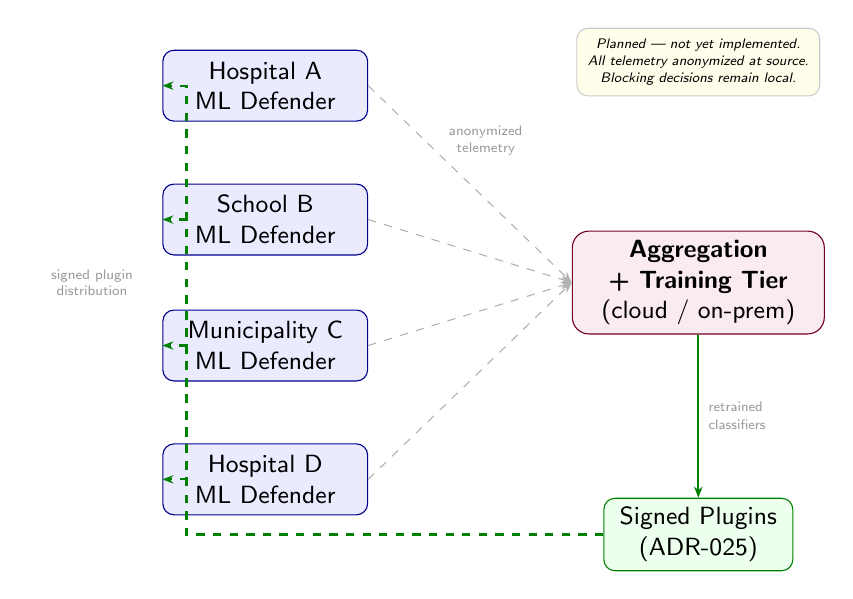
\begin{tikzpicture}[
            node_box/.style={rectangle, rounded corners=4pt, draw=blue!55!black, fill=blue!8,
            minimum width=2.6cm, minimum height=0.9cm, align=center, font=\small\sffamily},
            central/.style={rectangle, rounded corners=6pt, draw=purple!60!black, fill=purple!8,
            minimum width=3.2cm, minimum height=1.1cm, align=center, font=\small\sffamily},
            plugin_box/.style={rectangle, rounded corners=4pt, draw=green!50!black, fill=green!7,
            minimum width=2.4cm, minimum height=0.8cm, align=center, font=\small\sffamily},
            tel/.style={-{Stealth[length=4pt]}, dashed, gray!60},
            dist/.style={-{Stealth[length=4pt]}, thick, green!50!black},
            label_style/.style={font=\tiny\sffamily, gray!80}
        ]

            % Deployed nodes (left column)
            \node[node_box] (h1) at (0,  2.5) {Hospital A\\ML Defender};
            \node[node_box] (h2) at (0,  0.8) {School B\\ML Defender};
            \node[node_box] (h3) at (0, -0.8) {Municipality C\\ML Defender};
            \node[node_box] (h4) at (0, -2.5) {Hospital D\\ML Defender};

            % Central aggregation
            \node[central]  (agg) at (5.5, 0)  {\textbf{Aggregation}\\\textbf{+ Training Tier}\\(cloud / on-prem)};

            % Plugin distribution
            \node[plugin_box] (plugins) at (5.5, -3.2) {Signed Plugins\\(ADR-025)};

            % Telemetry arrows (anon)
            \foreach \n in {h1,h2,h3,h4} {
                \draw[tel] (\n.east) -- (agg.west)
                node[near start, above, label_style] {};
            }

            % Annotation on telemetry
            \node[label_style, align=center, text width=1.6cm] at (2.8, 1.8) {anonymized telemetry};

            % Plugin distribution arrows
            \draw[dist] (agg.south) -- (plugins.north) node[midway,right,label_style]
                {\shortstack[l]{retrained\\classifiers}};
            \foreach \n in {h1,h2,h3,h4} {
                \draw[dist, dashed] (plugins.west) -| (-1.0, 0) |- (\n.west);
            }
            \node[label_style, align=center, text width=1.4cm] at (-2.2, 0)
                {signed plugin distribution};

            % Privacy note
            \node[draw=gray!40, fill=yellow!8, rounded corners, font=\tiny\sffamily,
                inner sep=4pt, align=center] at (5.5, 2.8)
                {\textit{Planned --- not yet implemented.}\\
            \textit{All telemetry anonymized at source.}\\
            \textit{Blocking decisions remain local.}};

        \end{tikzpicture}
        \caption{Planned federated distributed intelligence architecture (\emph{not yet implemented}).
        Each deployed ML Defender node operates fully autonomously; anonymized flow-level telemetry
        is contributed to a central aggregation tier for periodic retraining. Updated classifiers
        are packaged as Ed25519-signed plugins (ADR-025) and distributed to the fleet. All detection
        and response decisions remain local to each node; no live network metadata leaves the
        deployment site. This architecture is a post-pipeline-stabilization milestone; a future
        revision of this paper will document the implementation.}
        \label{fig:federated}
    \end{figure}

    \textbf{11.16 Wazuh/NIST Integration (FEAT-INT-1).}
    Raw TCP streaming from Wazuh agents~\cite{wazuh2024} and NIST-aligned
    scanners into \texttt{rag-ingester} for composite attack graph correlation.
    Protocol design, motivation, and architectural constraints documented in
    \S\ref{sec:integration:philosophy}. Requires ADR-028 (RAG Ingestion Trust
    Model). Deferred to post-PHASE-2 pipeline stabilization.

    \textbf{11.17 Hardened Deployment Variants (ADR-030, ADR-031).}
    \label{sec:future:hardened}
    Two hardened deployment variants are documented as architectural decisions, both
    targeting a stronger kernel security posture:

    \textbf{ADR-030 (aRGus-AppArmor-Hardened):} Debian~13 + Linux~6.12~LTS +
    AppArmor enforcing mode. Full eBPF/XDP pipeline preserved. Compatible with ARM64
    (Raspberry Pi~4/5) and x86-64. This is the planned production-hardened variant,
    providing mandatory access control against confused-deputy attacks on plugin
    loading (motivated by the analysis of Hugo V\'azquez Caram\'es). Activation:
    post-PHASE-3 + hardware acquisition.

    \textbf{ADR-031 (aRGus-seL4-Genode):} Pure research variant on the seL4
    formally verified microkernel (${\sim}$12,000 lines of C verified in
    Isabelle/HOL). Linux runs as an unprivileged guest under Genode; XDP is
    infeasible in this model (no direct DMA access from guest), so libpcap is the
    mandatory capture fallback. The performance delta between eBPF/XDP and libpcap
    under seL4 is itself a measurable scientific contribution. Estimated overhead:
    40--60\%. Activation: post-ADR-030 + technical spike (2--3 weeks).

    Both variants will be validated in Vagrant first, then on bare-metal. Results
    will be published with measured honesty; ADR-031 will not be merged into
    \texttt{main} regardless of outcome.
    \textbf{11.18 Adversarial Capture-Retrain Loop (ACRL).}
    \label{sec:future:acrl}
    The out-of-distribution finding documented in \S\ref{sec:eval:xgboost:ood} motivates
    a production retraining methodology that does not depend on academic benchmark datasets.
    The proposed \emph{Adversarial Capture-Retrain Loop} (ACRL) operates as a closed cycle:
    (1)~a red team agent (initially MITRE Caldera~\cite{caldera2024} for deterministic
    ATT\&CK-mapped emulation; later a generative adversarial agent for adaptive evasion
    variants) executes attack techniques against an isolated network segment;
    (2)~the aRGus pipeline captures all resulting traffic via eBPF/XDP, producing
    ground-truth-labelled flows;
    (3)~the XGBoost plugin is retrained on the captured flows and re-evaluated against
    a held-out portion of the same session;
    (4)~the retrained model is signed (Ed25519, ADR-025) and hot-swapped without pipeline
    restart (ADR-026).

    The loop addresses the closed-world limitation identified in \S\ref{sec:limitations}
    (\textbf{10.13}): each retraining cycle expands the training distribution toward the
    real attack surface of the deployment environment. The architectural prerequisite ---
    hot-swappable signed plugins --- is already implemented and validated.

    Minimum scientific validity requirements for the ACRL data source: (i)~deterministic
    seed and versioned scenario for reproducibility; (ii)~ground-truth labels at flow
    granularity, derived from red team execution logs; (iii)~ATT\&CK tactic coverage
    across at minimum three families (volumetric, protocol-layer, application-layer);
    (iv)~network-valid traffic (correct TCP/IP headers, stateful handshakes);
    (v)~isolated sandbox with no production traffic contamination.
    The term \emph{Adversarial Capture-Retrain Loop} is introduced here as a named
    architectural pattern; related concepts include \emph{adversarial data flywheel}
    and \emph{red team loop}~\cite{sommer2010}. Implementation is tracked as
    DEBT-PENTESTER-LOOP-001 in the project backlog.

% ============================================================
    \section{Conclusion}
% ============================================================

    This paper presented ML Defender (aRGus NDR), an open-source network detection and response
    system built in C++20, designed from first principles to protect the organizations that need
    protection most and can afford it least.

    Evaluated against real botnet traffic from the CTU-13 Neris dataset --- traffic the system
    had never seen during training --- ML Defender achieves $\text{F1} = 0.9985$,
    $\text{Precision} = 0.9969$, and $\text{Recall} = 1.0000$. The two false positives are fully
    identified: an mDNS multicast frame and a broadcast frame, both generated by the VirtualBox host-only NIC.
    Their absence in bare-metal deployments is a reasonable expectation, but has not been empirically verified;
    bare-metal characterization remains Future Work~(\S\ref{sec:future:baremetal}). The
    Fast Detector alone produces a 6.61\% FPR on purely benign traffic; the ML Detector reduces
    this to zero real production blocks on the same corpus. End-to-end inference latency ranges
    from 0.24~$\mu$s to 1.06~$\mu$s per flow, entirely in-process, on commodity hardware costing
    approximately 150--200~USD.

    Under progressive load testing, the pipeline processes up to ${\sim}$34--38~Mbps --- the
    ceiling imposed by VirtualBox NIC emulation --- with zero packet drops, zero errors, and
    stable RAM (${\sim}$1.28~GB) across 2.37 million replayed packets. The bottleneck is the
    hypervisor, not the software.

    These results cover one botnet scenario from 2011. They demonstrate architectural viability
    and effective detection within that scope. The limitations in Section~\ref{sec:limitations}
    are the honest documentation of a system that does what it claims to do within the boundaries
    where it has been tested.

    A subsequent evaluation (DAY~122) integrated XGBoost~3.2.0 as a hot-swappable plugin and
    conducted a rigorous temporal holdout study on CIC-IDS-2017. The in-distribution results
    (Precision$=0.9945$, Recall$=0.9818$) confirm that the plugin architecture performs as
    designed. The out-of-distribution finding --- that no threshold satisfies both medical gates
    on Wednesday data, because application-layer DoS attacks are structurally absent from the
    training days --- is reported not as a failure but as a contribution: a quantified,
    empirically grounded argument for why production NDR classifiers must be trained on traffic
    from their actual deployment environment. The Adversarial Capture-Retrain Loop
    (\S\ref{sec:future:acrl}) is the architectural response.

    ML Defender was built because a friend lost his business to ransomware, and because a
    hospital in Barcelona was paralyzed by an attack on the same day its author was leaving a
    regional hospital in Extremadura --- the hospital that had diagnosed his porphyria and saved
    his life. The design constraints that followed from those two events were not abstract:
    open-source, commodity hardware, real-time response. Not a forensic tool. Not a dashboard. A
    system that acts.

    The \emph{Consejo de Sabios} represents a new mode of engineering: one that gives a single
    independent researcher access to the kind of multi-expert peer review that has historically
    required institutional affiliation, research groups, and geographic proximity to centers of
    expertise. The \emph{Test Driven Hardening} methodology that emerged from this collaboration
    has proven effective against some of the most subtle concurrency and memory bugs in the
    codebase.

    Both contributions --- the technical system and the collaborative methodology --- are acts of
    democratization. The parallel is not accidental. It is the point.

    \medskip

    \noindent For the hospital in Extremadura. For the friend whose business was broken by
    ransomware. For every small organization that has been told, implicitly or explicitly, that
    enterprise-grade security is not for them.

    \medskip

    \noindent \textit{It is now.}

% ============================================================
    \section{Reproducibility and Artifact Availability}
    \label{sec:reproducibility}
% ============================================================

    All experiments are reproducible from the public repository:
    \url{https://github.com/alonsoir/argus}

    \paragraph{Dataset Setup.}
    \begin{lstlisting}[language=bash]
# CTU-13 Neris (scenario 10) -- required for F1 validation
wget https://mcfp.felk.cvut.cz/publicDatasets/CTU-Malware-Capture-Botnet-42/\
botnet-capture-20110810-neris.pcap -O /vagrant/datasets/ctu13/neris.pcap
# Mirror: https://www.stratosphereips.org/datasets-ctu13

# CTU-13 bigFlows -- required for stress test
wget https://mcfp.felk.cvut.cz/publicDatasets/CTU-Malware-Capture-Botnet-42/\
bigFlows.pcap -O /vagrant/datasets/ctu13/bigFlows.pcap
    \end{lstlisting}

    \paragraph{F1 Evaluation.}
    \begin{lstlisting}[language=bash]
make pipeline-stop && make logs-lab-clean && make pipeline-start && sleep 15
make test-replay-neris
python3 scripts/calculate_f1_neris.py \
  /vagrant/logs/lab/sniffer.log --total-events 19135
    \end{lstlisting}

    \paragraph{Stress Test.}
    \begin{lstlisting}[language=bash]
vagrant ssh client -c "sudo tcpreplay -i eth1 --mbps=100 --loop=3 \
  /vagrant/datasets/ctu13/bigFlows.pcap"
    \end{lstlisting}

    \paragraph{Determinism.}
    Classifiers embedded in binary; no stochastic inference components; feature extraction
    deterministic. F1=0.9985 confirmed stable at total\_events = 12,563 / 12,605 / 12,723 /
    13,930.

% ============================================================
    \section*{Acknowledgments}
    \label{sec:acknowledgments}
% ============================================================

    This work was carried out independently, without institutional funding, without a research
    group, and without affiliation to any university or laboratory.

    The author engaged eight large language models --- Claude (Anthropic), Grok (xAI), ChatGPT
    (OpenAI), DeepSeek, Qwen (Alibaba), Gemini (Google), Kimi (Moonshot AI), and Mistral
    (Mistral AI) --- as structured intellectual collaborators across 132 days of continuous
    development. Their contributions to
    architectural decisions, failure mode identification, debugging, test scenarios, and paper
    review are documented in the project's commit history and ADRs. The \emph{Test Driven
    Hardening} methodology documented in Section~\ref{sec:consejo} emerged directly from this
    collaboration.

    This paper discloses AI involvement openly and precisely. The author remained the final
    arbiter of all decisions; all empirical validation was performed by the human author.

    The author wishes to acknowledge the friend whose business was destroyed by ransomware ---
    who will recognize himself in these pages. And the Hospital Universitario de Badajoz, Extremadura, whose
    physicians diagnosed a rare disease and gave the author the years needed to build something
    worth building. Thank you Pedro Risco and Agustín Pijierro.

    \medskip
    \noindent This work is dedicated to every hospital, school, and small organization that has
    ever been told that enterprise-grade security is beyond their reach.

% ============================================================
% Bibliography
% ============================================================

    \bibliographystyle{plainnat}
    \bibliography{references}

\end{document}